\documentclass[11pt]{article}
\usepackage{geometry}                
\geometry{letterpaper}                   

\usepackage{graphicx}
\usepackage{amssymb}
\usepackage{epstopdf}
\usepackage{xcolor}
\definecolor{ethblue}{RGB}{105, 132, 179}
\usepackage[colorlinks=true,allcolors=ethblue]{hyperref}

\usepackage{natbib}
\usepackage{siunitx}
\usepackage{xcolor}
\usepackage{subfigure}
\usepackage{caption}
\usepackage{float}
\usepackage[section]{placeins}
\usepackage[font=footnotesize,labelfont=bf]{caption}

\usepackage{amssymb, amsmath}
\DeclareMathOperator{\sign}{sign}
\DeclareGraphicsRule{.tif}{png}{.png}{`convert #1 `dirname #1`/`basename #1 .tif`.png}
\graphicspath{ {./images/} }
\setlength{\abovecaptionskip}{0pt}

\newcommand{\subfigimg}[3][,]{%
  \setbox1=\hbox{\includegraphics[#1]{#3}}% Store image in box
  \leavevmode\rlap{\usebox1}% Print image
  \rlap{\hspace*{10pt}\raisebox{\dimexpr\ht1-2\baselineskip}{#2}}% Print label
  \phantom{\usebox1}% Insert appropriate spcing
}


\setlength{\parindent}{0pt}
\setlength{\parskip}{0.6\baselineskip}
\usepackage{setspace}
\setstretch{1.25}


%\title{Title}
%\author{Name 1, Name 2}
%\date{date} 

\begin{document}
\pagenumbering{gobble} 



\thispagestyle{empty}

\begin{center}

\includegraphics[width=5cm]{ETHlogo.eps}

\bigskip


\bigskip


\bigskip


\LARGE{ Complex Social Systems:\\ }
\LARGE{Multi-dimensional opinion dynamics \\}

\bigskip

\bigskip

\small{Project Report}\\

\bigskip

\bigskip

\bigskip

\bigskip


\begin{tabular}{|c|}
\hline
\\
\textbf{\LARGE{Modelling Multi-dimensional }}\\
\\
\textbf{\LARGE{Opinion and Polarization Formation}} \\
\\
\hline
\end{tabular}
\bigskip

\bigskip

\bigskip

\LARGE{Michael Andres, Florian Dorner, Gian Luca Gehwolf, Fabian Hafner, David Metzger}



\bigskip

\bigskip

\bigskip

\bigskip

\bigskip

\bigskip

\bigskip

\bigskip

Zurich\\
December 2020\\

\end{center}



\newpage

%%%%%%%%%%%%%%%%%%%%%%%%%%%%%%%%%%%%%%%%%%%%%%%%%

\newpage


\section*{Abstract}
We investigate multi-dimensional opinion and polarization formation in networks of agents, both with and without the presence of social bots. We reproduce and generalize two models featuring opinion formation based on weighted balance theory (WBT), as well as the coevolution of social networks and opinion dynamics, respectively. In computational experiments we explore the effects of various modelling assumptions and the robustness of model behaviour to parameter changes. Both the precise form of the network evolution dynamics and the extent of "evaluative extremeness" determining how much people are influenced by others' opinions play an important role: With high level of evaluative extremeness, we observe strong polarization along a single axis of disagreement but opinions become more diverse if network ties are restricted to others with similar opinions. The effect of social bots is similarly modulated by the network: While bots spreading extreme opinions can increase polarization and bots with more neutral messaging can foster moderation, both are most effective if placed in highly connected nodes. Correspondingly, the effectiveness of bots greatly suffers if network ties are restricted to nodes with similar opinions. 
\section*{Agreement for free-download}

\begin{figure}[h]
    \centering
    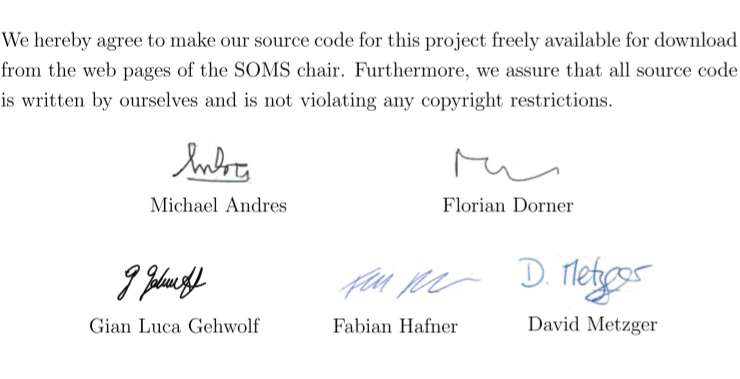
\includegraphics[width = 0.97\textwidth]{images/agreement_for_free_download.png}
    \label{dec_of_orig1}
\end{figure}


\newpage

\begin{figure}
    \centering
    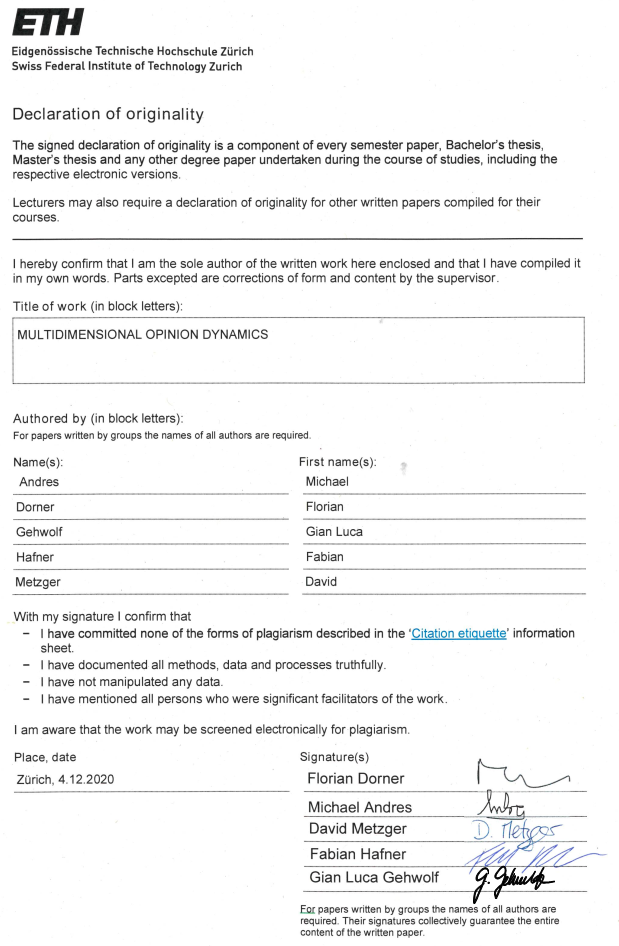
\includegraphics[width = 0.95\textwidth]{images/dec_of_origin.png}
    \label{dec_of_orig2}
\end{figure}


\newpage


{
  \hypersetup{linkcolor=black}
  \tableofcontents
}

\newpage


\pagenumbering{arabic}

\section{Individual contributions}

Florian Dorner proposed the abstract structure of the generalized model, contributed the initial implementation of the abstract generalized model and conducted and wrote about the experiments on bots. Fabian Hafner implemented the reproduction of the Weighted Balance Model, investigated the properties of the Generalized WBT Model and conducted the corresponding experiments. Gian Luca Gehwolf conducted a extensive literature review, wrote the introduction and motivations section, contributed to the implementation section, and commented and gave feedback to the coding of the models. David Metzger conducted the experiments for the coevolution model and contributed to the corresponding sections, as well as some parts of the Generalized Model. He also restructured the code for easier reproducibility. Michael Andres introduced a simplified structure to the implementation of the Generalized Model, reviewed and commented the code, conducted analysis of the network structures in gephi and took the lead in writing the summary.

Everyone proofread the report and contributed a variety of small improvements through their feedback. 

\section{Introduction and Motivations}

The divergence of opinions on certain issues can lead to the formation of several conflicting or contrasting groups. The (re-)emergence of populism in certain countries in Europe and in the US has led to divided societies with strongly opposing opinions on various issues. This political polarization in democratic societies has reached a point, where it poses a threat to political stability \citep{abramowitz2008,hare2014}. In the field of sociology, studies on dynamics of opinion formation have a long history. Additionally, the physics community has also contributed to this field, where studies on social networks and the dynamics of networks have been performed \citep{helbing1994,laguna2004,hegselmann2002,holme2006nonequilibrium}.

\citet{holme2006nonequilibrium} developed a model that combines opinion dynamics with assortative network formation. They argue that individuals can become like-minded because they are connected via the network, but at the same time they can also form a connection in network because they are like-minded. Previous models only accounted for one or the other \citep{castellano2003incomplete,deffuant2002can,liggett2012interacting,castellano2000nonequilibrium,mcpherson2001birds,sood2005voter,sznajd2000opinion}. Holme and Newman's dynamic, non-equilibrium model reaches a consensus state within a finite time and the authors analyze the distribution of community sizes in the converged model. They find a phase transitions in their model such that fundamental changes in the social structure of the community can sometimes be caused by small changes in the parameters of the system.
One limitation of Holme and Newman's model is that opinions are modeled as unidimensional. This can be problematic, as opinions about different topics are not always strongly correlated and people care more deeply about certain issues than others \citep{krosnick1990}. 

Still, opinion dynamic models that try to account for polarization, defined as "division into two conflicting or contrasting groups" (American Heritage Dictionary, 2011), have mostly focused on one-dimensional opinion models (\citep{lorenz2007,flache2017,jager2005,salzarulo2006}). On the other hand, there exist only a few multidimensional opinion dynamics models \citep{huet2010,flache2008,flache2011,schweighofer2020}. All these models can only generate a form of polarization under special conditions, such as high correlation of demographic attributes or complex social structures, with the exception of the model developed by \citet{schweighofer2020} which does not assume any underlying complex social or logical structures. With their Weighted Balance Theory (WBT) model, they are able to produce hyperpolarization: the emergence of opinion extremeness (opinions far away from the center) and issue constraint (positions on different issues strongly correlate, \citep{converse1964}). In the model, opinion change is induced through two modes: cognitive (issue positions) and affective components (interpersonal attitude), both influencing each other dynamically, e.g. human beings tend to agree more with people they like, and conversely they tend to disagree with people they dislike. However, the model is based on a strong approximation and assumes that each opinion on an issue contributes equally to the interpersonal attitude towards an other individual. As previously described, this contradicts Krosnick's (\citeyear{krosnick1990}) idea that some people care more deeply about certain issues and less about others. Additionally, \citet{schweighofer2020} mention that although their model does not require complex network structures to generate polarization, complex network structures can play a role in polarization dynamics, which previous models have already shown \citep{deffuant2013,Manzo2015,Hofstede2018}.

Opinion dynamics can also be influenced by factors other than actors and their networks. Artificial actors, also known as social bots, can have an impact on opinion dynamics. By deliberately trying to inflate the importance of certain topics via social media platforms such as Instagram, Twitter, or Facebook, bots have tried to influence recent presidential election campaigns in the US, France, and to a lesser extent in Germany \citep{kupferschmidt2017,bohannon2017}. There exist a few opinion dynamic models that account for the influence of bots \citep{ross2019,stella2018bots,el2018}. These models all show that bots have a significant impact on opinion dynamics. \citet{ross2019} and \citet{el2018} highlight that only a small number of bots is needed to influence opinion dynamics. \citet{stella2018bots} provide evidence that social bots target mainly human influencers but generate semantic content depending on the polarized stance of their targets. 

In this project, we study what effects network structures have on opinion polarization formation given that the WBT model developed by \citet{schweighofer2020} does not account for it. To achieve this, we combine the WBT model with the coevolution model developed by \citet{holme2006nonequilibrium}. This combined model we term "the generalised WBT model". Additionally, we simulate the effects of introducing bots in the generalised WBT model.

The remainder of this paper is structured as follows. Section \ref{modeldescr} first introduces the theoretical background of the opinion dynamic models developed by \citet{holme2006nonequilibrium} and \citet{schweighofer2020}. This is followed by a theoretical description of the generalised WBT model including the introduction of the bots to this model. Section \ref{impl} gives an overview on how we implemented our models in Python. In Section \ref{resanddis}, the results of our simulations using the different models are presented and discussed. In the final section, we summarise the results of our simulations, discuss the limitations of the models and give an outlook for possible future work. 


\section{Description of the Model} \label{modeldescr}
\subsection{First model: Coevolution of networks and opinions}\label{holme}
Our first model is based on \citet{holme2006nonequilibrium} and models the coevolution of opinions within a network of interacting people and the shape of the network. Each person in the network is modelled as one of the $N$ vertices in a simple undirected graph $G$ with $M$ edges representing connections between persons. Furthermore, each person has an opinion $o$ from a set of opinions $O$ which is stored in the vertex corresponding to the person.
\begin{figure}[h]

\begin{center}
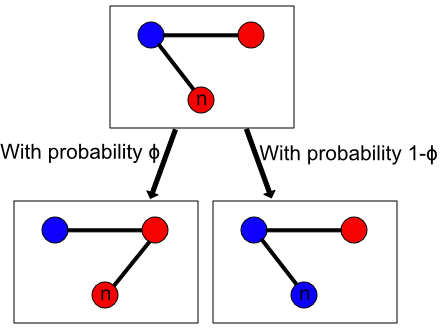
\includegraphics[width=0.4\textwidth]{coevo.png}
\end{center}
\caption{Dynamics of the basic coevolution model}
\label{Coevo}
\end{figure}
The graph $G$ is initialized with edges and opinions sampled uniformly and the dynamics work as depicted in Figure \ref{Coevo}: At each time step $t$, a vertex $n$ is picked at random. If it has degree zero (no connections to other nodes), nothing happens. Else, with probability $\phi$, a random edge connected to $n$, $(n,m)$ is selected and changed to $(n,m')$ where $m'$ is a vertex with the same opinion as $n$, thus $o(m')=o(n)$. If no such $m'$ exists, nothing happens. In other words, $n$ gives up an old connection to connect to someone with the same opinion. Otherwise, with probability $1-\phi$, a random vertex $l$ that is directly connected to $n$ by an edge is selected and $n$'s opinion $o(n)$ is set to $o(l)$. This means that $n$ changes their opinion to the opinion of one of their connections. Once all vertices in a connected component of $G$ have the same opinion, the opinions of all vertices $n$ in the component stay fixed as none of the vertices is connected or can connect to a vertex $m$ with a different opinion $o(m)\neq o(n)$. Thus convergence of opinions is achieved once opinions are constant on every connected component. We call the order of a connected component community size and denote it by $s$, while the largest community size is denoted by $S$.

\FloatBarrier
\subsection{Second model: Weighted Balance Theory}
\label{wbt_descr}

The second model we studied is based on the Weighted Balance Theory (WBT) developed by \citet{schweighofer2020}. In this paper, the authors try to explain the simultaneous emergence of the socio-political phenomena of opinion extremeness and issue constraint\footnote{referring to the perceived correlation between opinions on different topics.}, which they call \textit{hyperpolarization}. In the case of hyperpolarization, two groups of agents with diametrically opposed opinion vectors emerge. This can be compared e.g. to a two-party system splitting the population into 'conservative' and 'liberal' clusters. 

The paper models the opinions of agent $i$ as vector 
\[
\mathbf{o}(i) = \begin{pmatrix} 
o_1(i) \\
\vdots \\
o_D(i)
\end{pmatrix}
\in [-1,1]^{D}
\]
where $D$ is the total number of opinions. Each entry represents the opinion about a certain topic and can range from complete opposition (represented by -1) to complete support (represented by +1).

The WBT model is based on the work on Balance Theory by \citet{heider1946}, which focuses on the simpler cases of a single dimensional opinion vector with categorical value $\pm 1$. Balance Theory proposes a 'triad' of two agents, which describes their opinion about a certain topic $o_d(i)$, $o_d(j)$ and their interpersonal attitude $A_{ij}$. This triad is is called \textit{balanced}, whenever either both persons support the issue and have a positive attitude to each other, or have a negative attitude of each other and disagree about the policy issue. If positive opinions are encoded as $1$ and negative ones as $-1$, the triad is thus balanced whenever the product of the persons' opinions about the policy is equal to their attitude about each other or equivalently the product of both opinions about the policy and the interpersonal attitude is 1.

The WBT model now expands upon this construct. Instead of the product, WBT uses the signed geometric mean

\[\text{SGM}(x,y):=\sign(xy)\sqrt{(|xy|)}\] 

to account for continuous opinions and ensure that issue-induced interpersonal attitudes have similar strength as the opinions about the issue. 

In the case of multidimensional opinions about a set of issues $D$\footnote{We refer to the set of opinions as $D$ as well as to that set's cardinality.}, the interpersonal attitude of agent $i$ about person $j$ and vice versa is calculated as a monotonously growing transformation $f$ of the arithmetic mean

\[A_{ij}:=f\left(\frac{1}{D}\sum_{d=1}^{D}\text{SGM}(o_{d}(i),o_{d}(j))\right).\] 

The functional form of $f$ is chosen to preserve the sign to reflect peoples' tendency to agree with people they like and disagree with those they do not like -- with the second relation often referred to as the backfire-effect \citep{wood2019elusive,bail2018exposure}. Empirical evidence from survey data for the 2016 US presidential election suggests a roughly sigmoidal form \citep{schweighofer2020}, such that
$f$ is chosen to be

\[
f(x) = \sign{(x)}|x|^{1-e}
\]

where the free parameter $e$ is called \textit{evaluative extremeness} and determines how strongly small amounts of (dis-)agreement are reflected in peoples' displayed attitude towards each other. It is worth noting that $A_{ii} \neq 1$ is possible.

Opinions are initialized uniformly randomly in $[-1,1]$ for every agent $i$ and every component $o_d(i)$ of the respective opinion vector $\mathbf{o}(i)$. Then, in each model step, we iterate over all agents in random order and for each agents $i$ another agent $j$ is sampled. Then, the interpersonal attitude $A_{ij}$ is calculated and an agent $i$ incrementally adjusts their opinion about issues $o(i)$ to better match the balance dictated by Weighted Balance Theory by slowly adjusting each of their opinions contained in the vector $\mathbf{o}(i)$ towards the optimally balanced state 

\[ 
\mathbf{b}^{ij} := \begin{pmatrix} 
{b}^{ij}_1  \\
\vdots \\
{b}^{ij}_D
\end{pmatrix} :=
\begin{pmatrix}
\text{SGM}(o_1(j),A_{ij})  \\
\vdots \\
\text{SGM}(o_D(j),A_{ij})
\end{pmatrix}
\]. 

The unilateral update is performed as 
\[ 
\mathbf{o}(i)\leftarrow  \mathbf{o}(i) + \alpha \left[\mathbf{b}^{ij}-  \mathbf{o}(i)\right]+\xi(0,z)
\]

with a fixed update parameter $\alpha$\footnote{\citet{schweighofer2020} state that it is reasonable to assume that opinions have a certain degree of inertia and do not change completely upon a single interaction with another person. This fact is represented by $\alpha$.} and noise $\xi(0,z)$ generated by a normal distribution with mean $0$ and standard deviation $z$. The random noise accounts for effects and influences not captured by the model and including it ensures robustness of our results. Agents will try to match the opinions about issues of people they like ($A_{ij}>0$) while tending to disagree about issues O of people they dislike ($A_{ij}<0$).
The algorithm is graphically shown for a simple case of a two-dimensional opinion vector in Figure \ref{fig:wb}.

\begin{figure}[htb]
    \centering
    \includegraphics[width=0.87\textwidth]{images/weighted_balance/wbt_model.pdf}
    \caption{Schematic of opinion exchange under the WBT model with $\alpha = 0.5$. Adapted from: \cite{schweighofer2020}}
    \label{fig:wb}
\end{figure}

The model is considered to have converged once the difference of the absolute entries of consecutive  opinion matrices
\[
O := 
\begin{pmatrix} 
\mathbf{o}(1)^\text{T}  \\
\vdots \\
\mathbf{o}(N)^\text{T}
\end{pmatrix}  \in [-1,1]^{D \times N}
\]
does not change significantly, or more formally:

\[
|O_t - O_{t-1}| := \sum_{i=1}^N \sum_{d=1}^D |o_d(i)| \leq \chi(N,D,z)
\]
where $\chi(N,D,z)$ is a threshold dependent on the number of agents $N$, number of opinions $D$ and standard deviation of the noise-level $z$. To control for robustness we require that at least 5 consecutive time steps meet this criterion. 

\subsection{Generalized Model}\label{general}
We propose a set of extensions to \citet{holme2006nonequilibrium}'s model: First, we replace the discrete opinions $o$ by a vector of continuous opinions $\mathbf{o}\in\mathbb{R}^{k}$ like in the WBT model. Then, the condition on the active node $n$'s opinion $o(n)$ and another node $m$'s opinion $o(m)$ for $m$ being included in the sampling of new connections can be generalized from the equality operator to a general map
\[
\text{connect}:\mathbb{R}^{k}\times\mathbb{R}^{k}\to\{0,1\}.
\] 

Similarly, the update of $o(n)$ based on a connected node $m$'s opinion $o(m)$ can be generalized from the projection of the second dimension \[\text{update}(o(n),o(m))=o(m)\] to a general (stochastic) map 
\[
\text{update}:\mathbb{R}^{k}\times\mathbb{R}^{k}\to \mathbb{R}^k.
\] 

Similarly, the initialization of opinions, the way 'active' nodes are sampled and the convergence criterion can be modified. 
\subsubsection{Generalized WBT model}

In particular, we can obtain the WBT model by setting $M={(N^2-N)}/{2}$ such that $G$ is fully connected, $\phi=0$, $\text{connect}$ arbitrary and


\[
\text{update}(\mathbf{o}(i),\mathbf{o}(j)) =  \mathbf{o}(i) + \alpha \left[\mathbf{b}^{ij}-\mathbf{o}(i)\right]+\xi(0,z).
\]

As the WBT model updates all its nodes in (a random) sequence rather than sampling nodes independently at each time step, we have to draw active nodes without replacement rather than independently at each step (starting over once no more nodes are left to be drawn) to match the WBT model's fine dynamics. Note that while \citet{schweighofer2020} refer to a whole pass through all nodes as a step, we choose to refer to a single node update as a step in the following for the sake of generality. 


This framing of the WBT model immediately suggests extensions to arbitrary graphs by keeping $\phi=0$ but reducing the amount of edges $M$ or initializing the graph $G$ with a specific structure. Similarly, by introducing a connection criterion and increasing $\phi$, the WBT model can be extended to dynamically changing graphs. The connection criterion could be based on a positive mutual opinion $A_{ij}$, matching signs for all opinion dimensions $o_d(i)$ and $o_{d}(j)$, a positive scalar product $\mathbf{o}(i)\cdot \mathbf{o}(j)$, or based on a threshold on the difference in opinions $|\mathbf{o}(i) - \mathbf{o}(j)| < \varepsilon(N,D,z)$. 

\subsection{Bots}
To investigate the effect of bots or other malicious actors that actively try to spread their opinion on the generalized Weighted Balance model, we consider three different bot models: In all three, bots work like normal nodes but we modify the update function, such that bots never change their opinions. In the first model, all bots have the same opinion at the extreme end of the spectrum meaning that $o_{d}(i)=1$ for all opinion dimensions $d$. The second model is like the first, but this time, bots act on both sides of the opinion spectrum such that half of the bots have $o_{d}(i)=-1$ for all opinion dimensions $d$, while the rest is on the other extreme, as before. In the third model, bots have neutral opinions on all topics such that $o_{d}(i)=0$ for all opinion dimensions $d$. Next, bots can either be placed in random nodes, or more selectively in the most (or least) connected nodes according to the degree. Furthermore, we consider both cases in which bots connect to other nodes in the same way all nodes do and cases, in which the bots' connect function is modified such that they sample their new connections from the full set of nodes rather than being restricted by the same connect function as other nodes. 

\section{Implementation} \label{impl}


All the opinion dynamics models in this work are implemented as agent-based models in \texttt{Python}. 
We implemented the generalized model described in subsection \ref{general} in \texttt{model.py} in the class \texttt{coevolution\_model\_general}. As all of the other models we considered are special cases of the model and were easily implemented as subclasses. \\
In the generalized model, the network graph is first initialized as a random graph with a predefined number of \textit{vertices} and \textit{edges} and a discrete or continuous opinion value attached to each node. The opinions of the \textit{vertices} and the \textit{edges} are updated in the  \texttt{step} function using the specific \texttt{update} and \texttt{connect} functions as specified in the respective subclasses. In a simulation run, the \texttt{step} function is repeated as long as the \texttt{converge} function, which is defined differently in each subclass, returns a false value indicating that the model has not converged. For some of our graphs, we also introduced a strict step limit to save time. 

\subsection{Coevolution of networks and opinion model}

The coevolution model is implemented as a subclass of \texttt{coevolution\_model\_general} called \texttt{holme} in \texttt{model.py}. In this subclass, we set the \texttt{update} and \texttt{connect} functions to
\[\text{update}(o(n),o(m))=o(m)\] and \[\text{connect}= [o(n)==o(m)]\] to match the behaviour of the coevolution model as described in section \ref{holme}. 


\subsection{Weighted Balance Theory Model}
While the Weighted Balance Theory model can easily be implemented as a subclass of \texttt{coevolution\_model\_general} as described in \ref{WBTgen} and we did this in \texttt{weighted balance}, we also provide a second simpler implementation in \texttt{WBT\_model.py} and verified that both versions produce the same behaviour. 

In both cases, we chose  
\[
\varepsilon(N,D,z) = NDz
\]
as convergence criterion, as described by \citet{schweighofer2020}. 

The simpler implementation can be run via the function $\text{run\_model}(N,D, e, z,\alpha)$ which, per default, computes time steps until the model converges. Alternatively, an opinion matrix $O$ and attitude matrix $A$ can be initiated and then each timestep can be calculated individually with the update function $\text{update\_model}(A, O, e, z, \alpha)$ function. Additionally, the hyperpolarization parameter can be calculated with the function $\text{H}(O)$. 


\subsection{Generalized WBT Model}\label{WBTgen}

Similar to the coevolution model, we constructed a subclass  \path{weighted_balance_general} in \path{model.py} for the generalized WBT model, which uses \[
\text{update}(\mathbf{o}(i),\mathbf{o}(j)) =  \mathbf{o}(i) + \alpha \left[\mathbf{b}^{ij}-\mathbf{o}(i)\right]+\xi(0,z)
\] and different \texttt{connect} functions. 

\subsection{Bots}
We built a subclass \path{weighted_balance_general} of \texttt{coevolution\_model\_general} to introduce bots. For this, we added a dummy dimension indicating whether a node is a bot to the opinion dimensions. Then, we modified the update function used in \ref{WBTgen} to keep the dummy dimension constant and ignore it for the calculation of the update, unless it is equal to $1$, in which case the updating node is a bot and the update function just returns the node's initial opinion (including the dummy dimension). Similarly, we modified the connect function to ignore the dummy variable.

However, the class also allows for changing the connect function and we experimented with setting connect to \texttt{TRUE} for all other nodes when the active node is a bot, such that bots sample their connections from all nodes rather than just ones with similar opinions. Furthermore, the class allows for various ways of setting bots' opinions and placing them in specific nodes, which are further explained in the code. 

While we only implemented bots in a dynamic graph setting akin to the generalized WBT model, the basic WBT model can be recovered by using a fully connected graph and $\phi=0$. Similarly, setting $\phi=0$ allows for a WBT model with bots on static graphs. 

Lastly, we adapted the convergence criterion to $\varepsilon(N,D,z) = (1-\phi)(N-N_{bots})Dz$  to account for the smaller expected change in the opinion matrix because of bots not changing their opinions and edge changes happening instead of opinion updates with probability $\phi$. 




\section{Simulation Results and Discussion} \label{resanddis}
\subsection{First model: Coevolution of networks and opinions}

\begin{figure}[!htb]
\minipage{0.30\textwidth}
\centering
  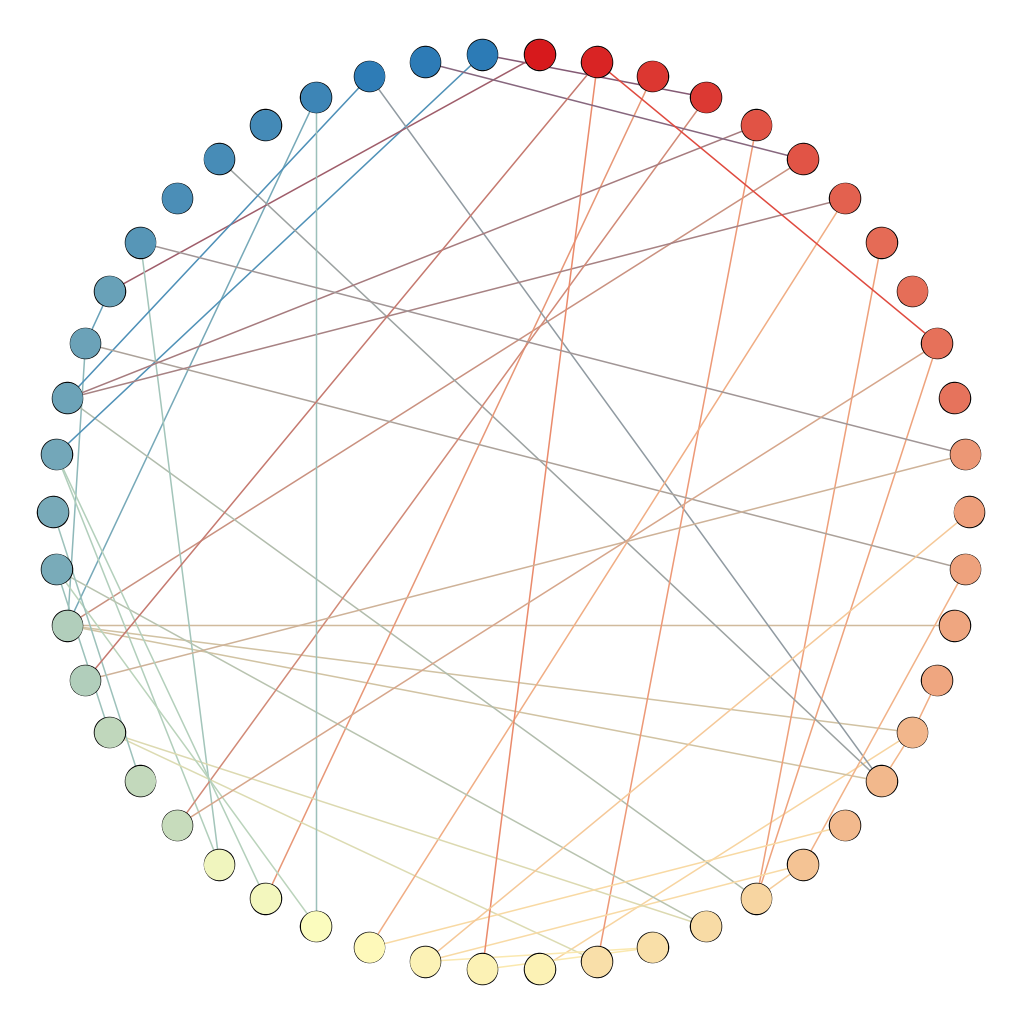
\includegraphics[width=0.95\linewidth]{images/Evolutions/Holme0.png}
  \caption*{Step 0}
  %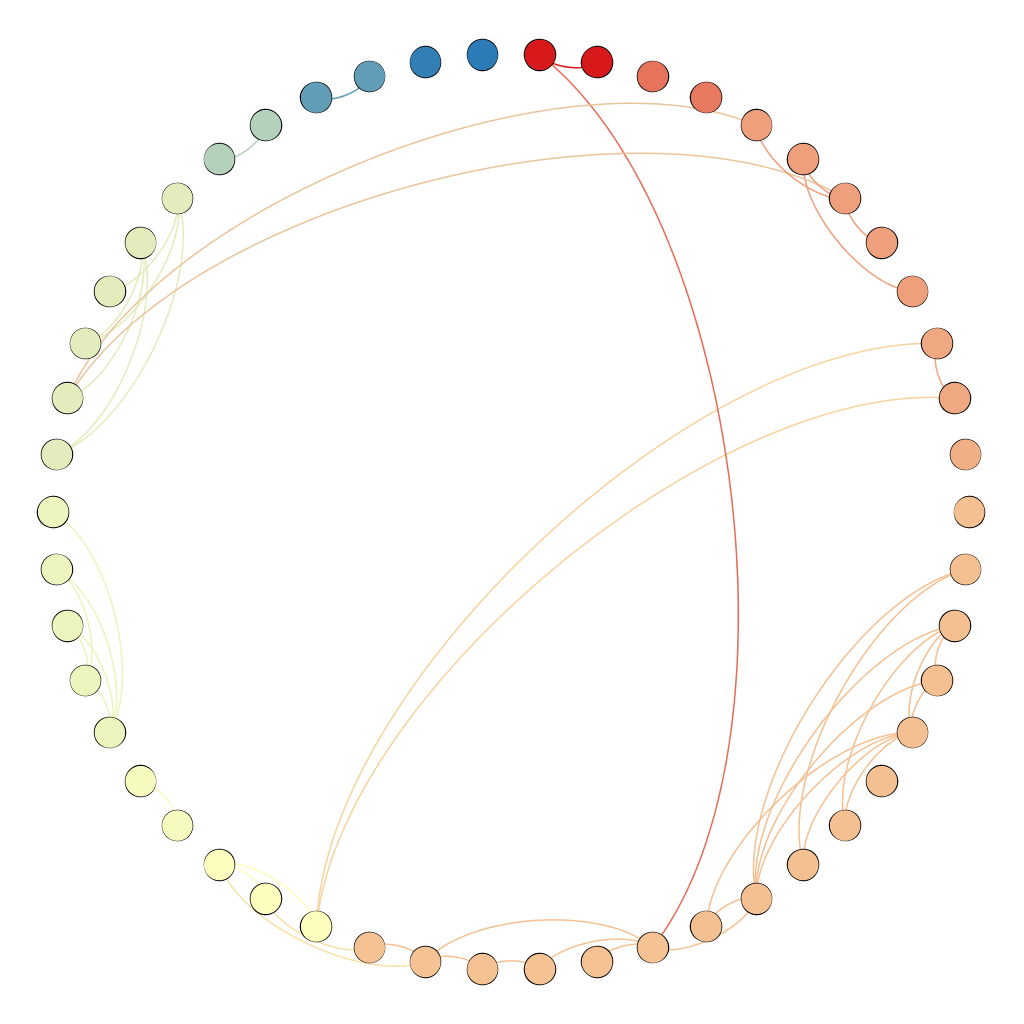
\includegraphics[width=0.7\linewidth]{images/Evolutions/Holme400.png}
  %\caption*{Step 400}
\endminipage\hfill
\minipage{0.30\textwidth}
\centering
  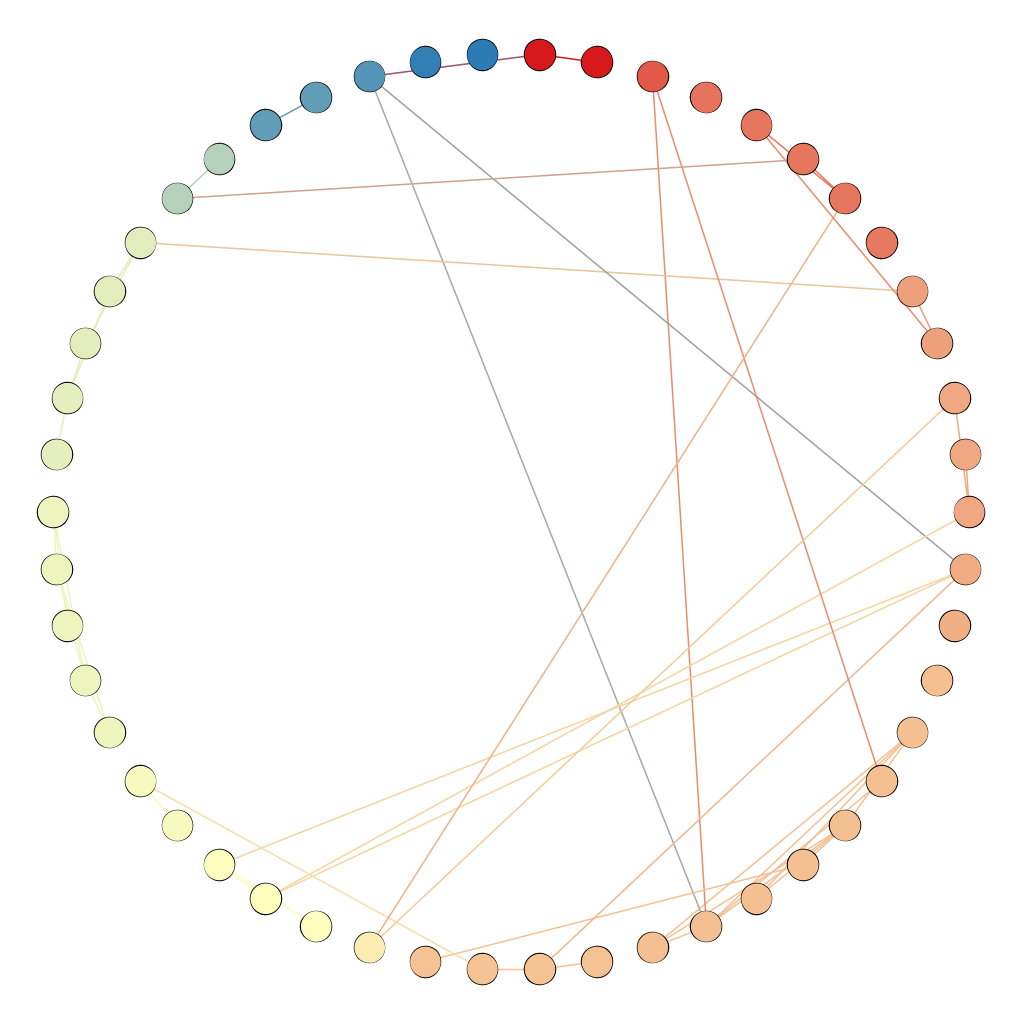
\includegraphics[width=0.95\linewidth]{images/Evolutions/Holme200.png}
  \caption*{Step 200}
\endminipage\hfill
\minipage{0.30\textwidth}
\centering
  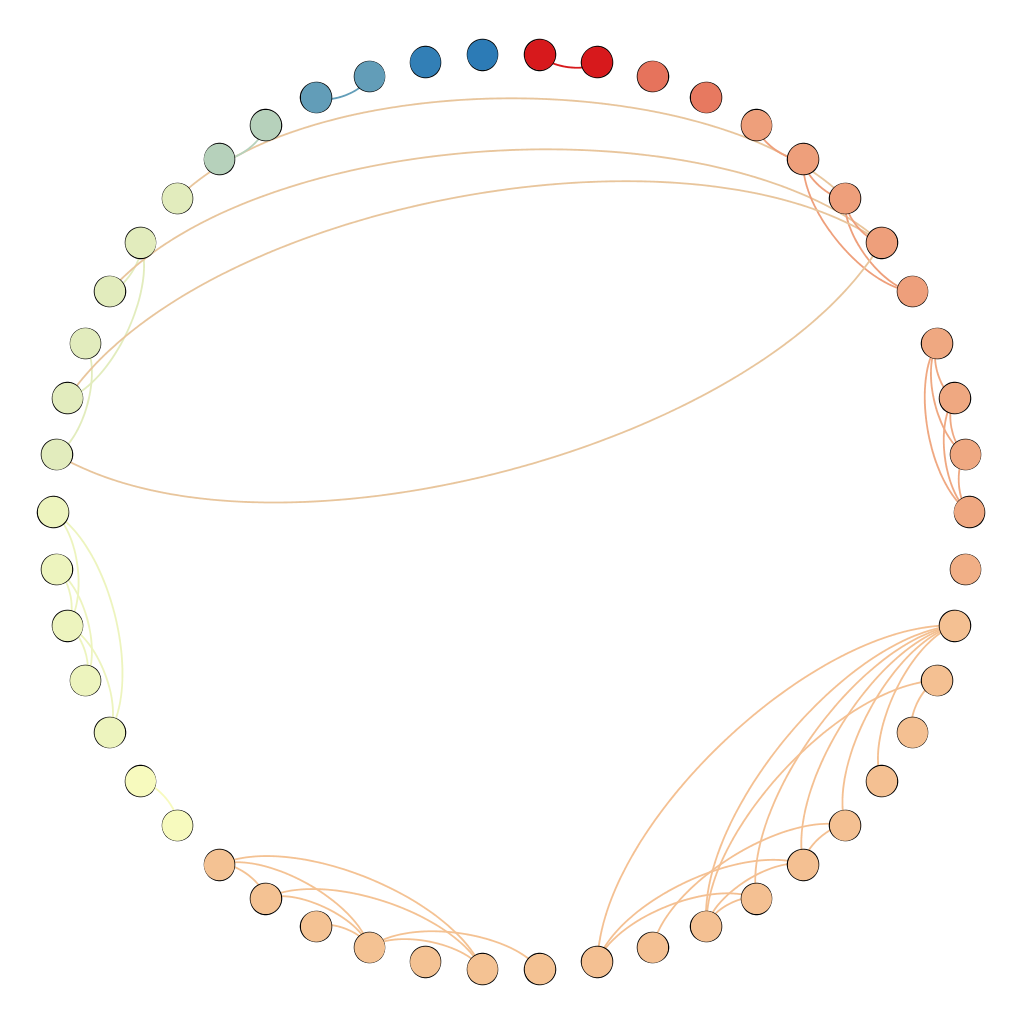
\includegraphics[width=0.95\linewidth]{images/Evolutions/Holme1000.png}
  \caption*{Step 1000}
\endminipage\hfill
\vspace{0.5cm}
\caption{Various Steps of the Holme Model with 50 nodes and 50 edges and with $\phi = 0.5$. Each node has one opinion which is represented by the color and placement in the circle, where blue and red are the relative extremes. Graphs are drawn with Gephi using the Circular Layout.}
\label{HolmeEvo}
\end{figure}

In their analysis, \citet{holme2006nonequilibrium} focus mainly on the community size $s$ given by the order of the connected components with internal consensus that form at convergence. They investigate how the community sizes are distributed and how they vary with the parameter $ \Phi $, i.e. relative frequency of opinion change vs. edge change. We attempted to reproduce their findings. In Figure \ref{HolmeEvo} we see an exemplary run in a small graph with $\phi = 0.5$, where multiple components emerge. Because of our limited computational resources, we had to reduce the size of the network compared to the original paper. Our results for the distribution of the community sizes in a graph with $640$ vertices were less smooth but qualitatively compatible with the results from the paper, which we can see in Figure \ref{holme1_dist}: for very small $\Phi$, i.e. for high edge change and low opinion change, we find configurations with one giant component and many small components, whose numbers decay exponentially with the size. For $\Phi$ around 0.46 we find more distributed sizes. They fit a power law for sizes between 8 and 80. In contrast to \citet{holme2006nonequilibrium} we frequently find giant components in the converged model. For $\Phi$ close to 1, where the opinions remain as initialized, the communities are formed by nodes with the same initial opinion. The resulting distribution is close to a multinomial distribution with a mean equal to $\gamma = 10$, the average number of nodes per opinion.

\begin{figure}[!htb]
\minipage{0.45\textwidth}
  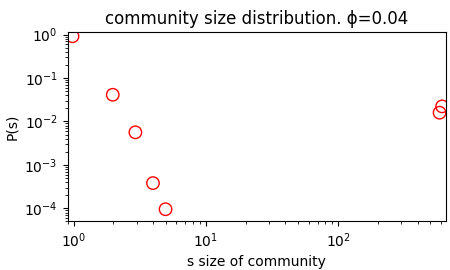
\includegraphics[width=\linewidth]{images/holme/size_distribution0.04s.png}
  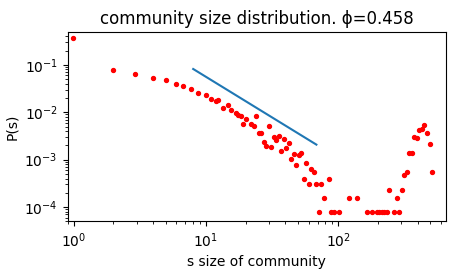
\includegraphics[width=\linewidth]{images/holme/size_distribution0.458s.png}
  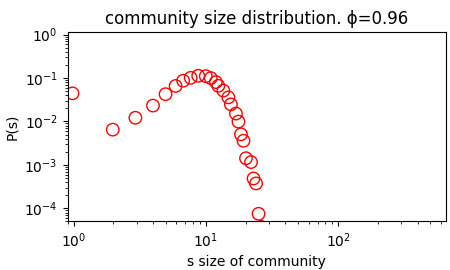
\includegraphics[width=\linewidth]{images/holme/size_distribution0.96s.png}
  
  \caption{Histograms of community sizes in the consensus state for different values of $\Phi$.  Distribution of the community sizes over $400$ iterations with $N=640$ vertices. $\gamma=10$, $k=4$}
  \label{holme1_dist}
\endminipage\hfill
\minipage{0.48\textwidth}
\centering
  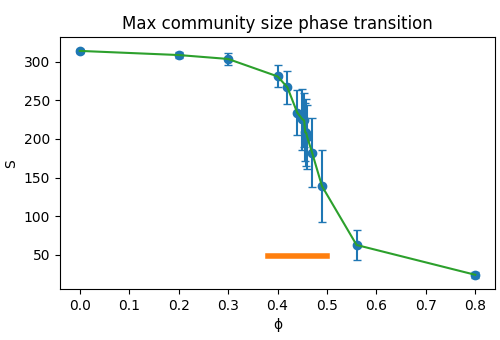
\includegraphics[width=\linewidth]{images/holme/maxS.png}
  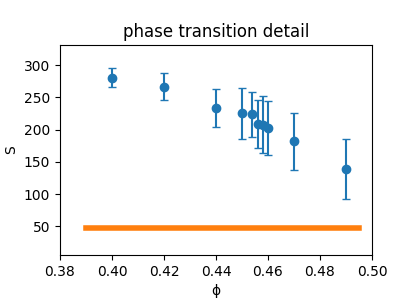
\includegraphics[width=0.8\linewidth]{images/holme/maxSdetail.png}
  
  \caption{Size of the largest community for different $\Phi$, average and standard error over $80$ iterations with $N=320$ vertices. $\gamma=10$, $k=4$}
  \label{holme2_phase}
\endminipage\hfill

\end{figure}

To take a closer look at the phase transition found by  \citet{holme2006nonequilibrium}, we ran the model for many different values of $\Phi$, which can be seen in Figure \ref{holme2_phase}. Around $\Phi = 0.45$ the model transitions from a consensus state where most individuals hold the same opinion to one where there is a diverse range of opinions in the population. 
\FloatBarrier
\subsection{Second model: Weighted Balance Theory}

To evaluate the extent of hyperpolarization in their model, \citet{schweighofer2020} suggest the hyperpolarization measure 

\[
H(O):=\frac{4}{N^2}\sum_{1=i<j}^{N}\left(\frac{\delta(o(i),o(j))}{ \delta_{\max}}\right)^2,
\] 
where $\delta$ denotes a metric (we use the euclidean metric) and $\delta_{max}$ is the maximal value of this metric for two points in the hypercube $[-1,1]^D$. In the case of maximal hyperpolarization\footnote{which can only happen with an even number of nodes}, we have $H(O)$=1: Without loss of generality, we can assume that the first $\frac{N}{2}$ nodes have opinion $1$ across all dimensions, while the rest of the nodes have opinion $-1$. Then, all terms in the sum are either $0$ if $i$ and $j$ are both larger or both smaller than $\frac{N}{2}$, or $1$ if they are on different sides of $\frac{N}{2}$. Because we only sum over terms with $i<j$, all terms with $i>{\frac{N}{2}}$ and all terms with $j<{\frac{N}{2}}+1$ fade and the sum reduces to \[\sum_{1=i<j}^{N}\left(\frac{\delta(o(i),o(j))}{ \delta_{\max}}\right)^2=\sum_{i=1}^{\frac{N}{2}}\sum_{j=\frac{N}{2}}^{N} 1=\left(\frac{N}{2}\right)^2=\frac{N^2}{4},\] such that $H(O)=1$ as claimed. On the other hand, $H(O)=0$ if and only if all nodes have the same opinion.  


First, we tried to reproduce the emergence of hyperpolarization under the conditions set in the original paper, which can be seen in Figure \ref{WBT_3D}. In this three-dimensional cube every dimension responds to an opinion $d_i$. This low-dimensional model already shows interesting behavior: After random sampling, the agents' opinions are initially drawn to the center $(0,0,0)$. However shortly after, two distinct groups of like minded agents begin to form, repulse each other and eventually end up in opposing corners of the cube. 


\begin{figure}[htb!]
  \centering
 \begin{tabular}{@{}p{0.33\linewidth}@{\quad}p{0.33\linewidth}@{\quad}p{0.33\linewidth}@{}}
    \subfigimg[width=\linewidth]{$t=1$}{images/weighted_balance/t1.pdf} &
    \subfigimg[width=\linewidth]{$t=22$}{images/weighted_balance/t22.pdf} &
    \subfigimg[width=\linewidth]{$t=60$}{images/weighted_balance/t60.pdf}
  \end{tabular}
  \caption{Weighted Balance Model with randomly sampled initial opinions and parameters $N=500$, $D=3$, $e=0.3$, $\alpha=0.4$, $z=0.01$. In the final time-step depicted the models shows a hyperpolarized state with $H \simeq 0.85$. The corners towards which the model converges are random, thus depending on the random starting conditions, the model always ends up converging into diametrically opposed stable states.}
  \label{WBT_3D}
\end{figure}


Next, in order to better understand the model behavior under parameter changes, we varied all parameters and plotted the resulting changes in hyperpolarization $H(O)$ in Figure \ref{ana_wbt}.
\begin{figure}[!h]
\begin{center}
\subfigure[Evaluative extremeness]{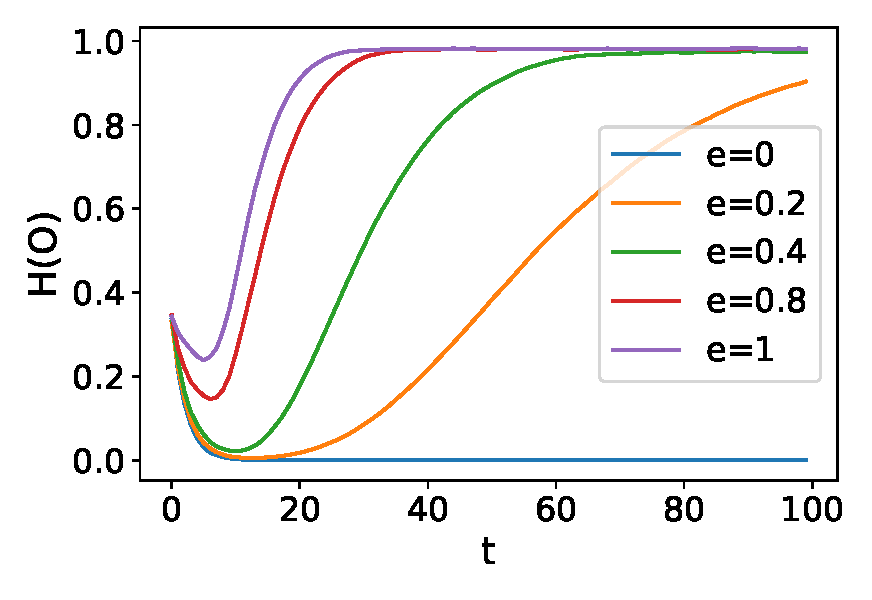
\includegraphics[width=0.49\textwidth]{images/weighted_balance/testing_e.pdf}}
\subfigure[Number of agents]{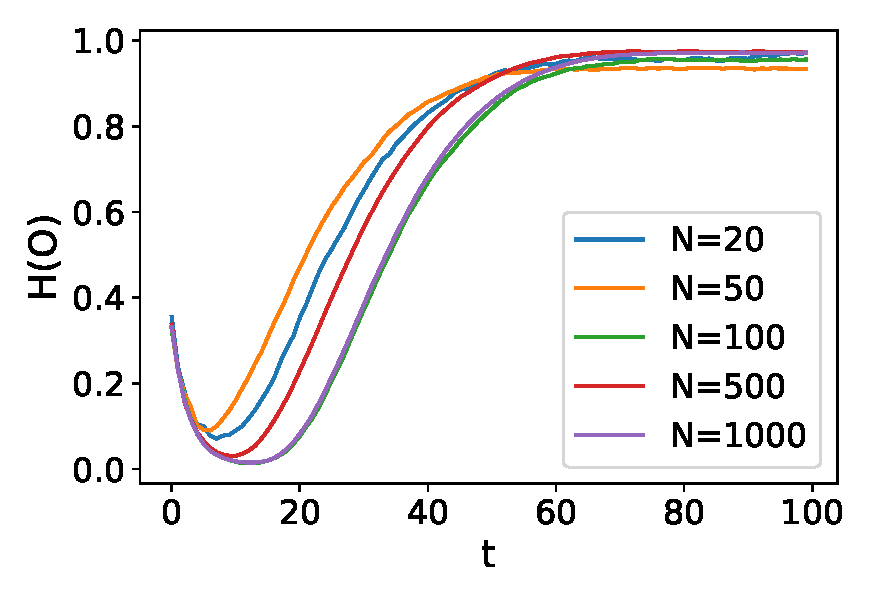
\includegraphics[width=0.49\textwidth]{images/weighted_balance/testing_N.pdf}}
\\
\subfigure[Opinion dimensions]{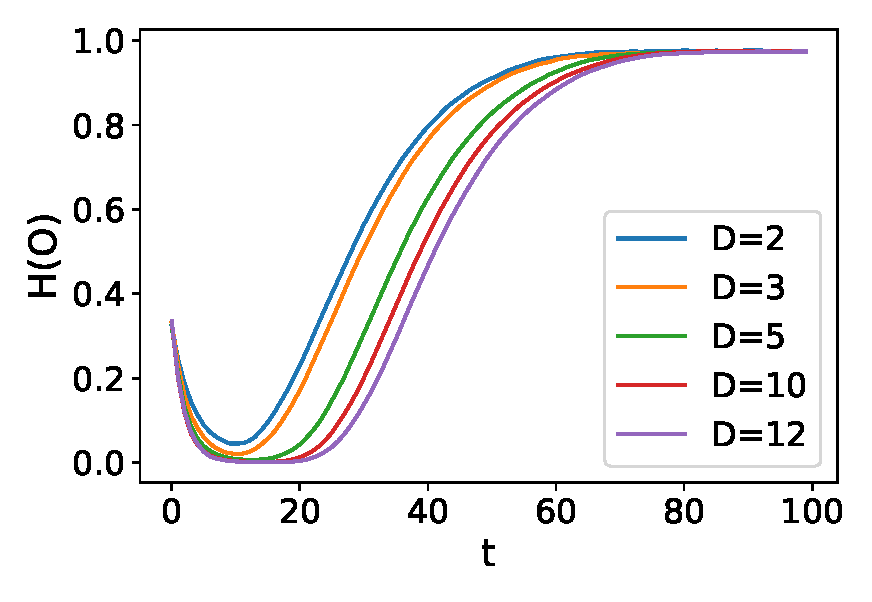
\includegraphics[width=0.49\textwidth]{images/weighted_balance/testing_D.pdf}}
\subfigure[Noise level]{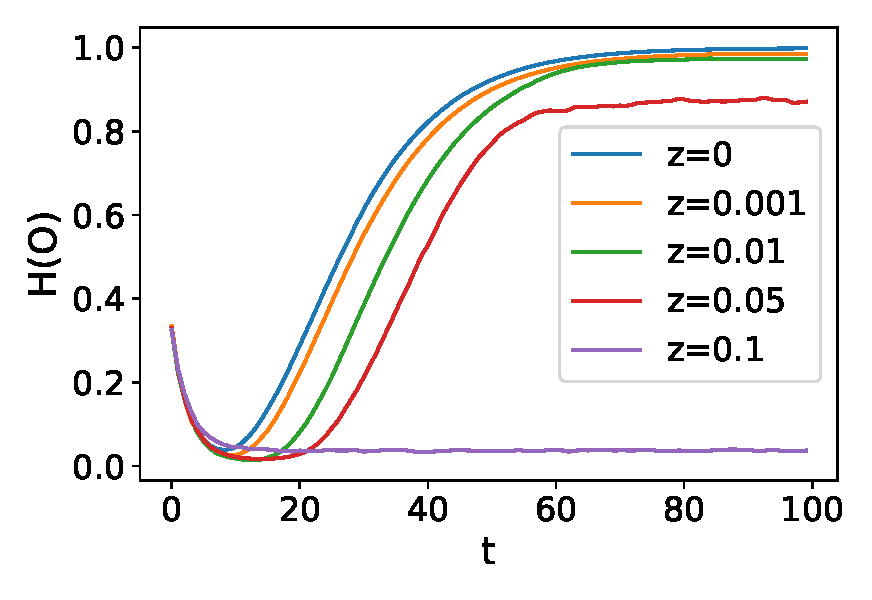
\includegraphics[width=0.49\textwidth]{images/weighted_balance/testing_z.pdf}}
\end{center}
\caption{Convergence behaviour to a hyperpolarized state for various variations of the parameter (a) $e$, values of $N=500$, $D=3$, $z=0.01$ and $\alpha=0.4$ kept constant; (b) $N$, values of $D=3$, $e=0.4$, $z=0.01$ and $\alpha=0.4$ kept constant; (c) $D$, values of $N=500$, $e=0.4$, $z=0.01$ and $\alpha=0.4$ kept constant; (d) $z$, values of $N=500$, $D=3$, $e=0.4$ and $\alpha=0.4$ kept constant. From these Figures one can see that the evaluative extremeness $e$ is the main driver of hyperpolarization. $N$ and $D$ have major influence on the convergence speed, while $z$ only produces complete hyperpolarization for $z \lesssim 0.05$.}
\label{ana_wbt}
\end{figure}

We observe that the qualitative behaviour does not fundamentally change for most parameter perturbations. Important exceptions are high values of the noise level $z$ and very low evaluative extremeness $e$, which was also highlighted by \citep{schweighofer2020} and can be seen in Figure \ref{WBT_Evo}. In the Figure we still see the polarization into two clusters, however due to the evaluative extremeness being 0, they do not drift towards the corners but rather stay close to the center.


\begin{figure}[htp!]
\minipage{0.24\textwidth}
  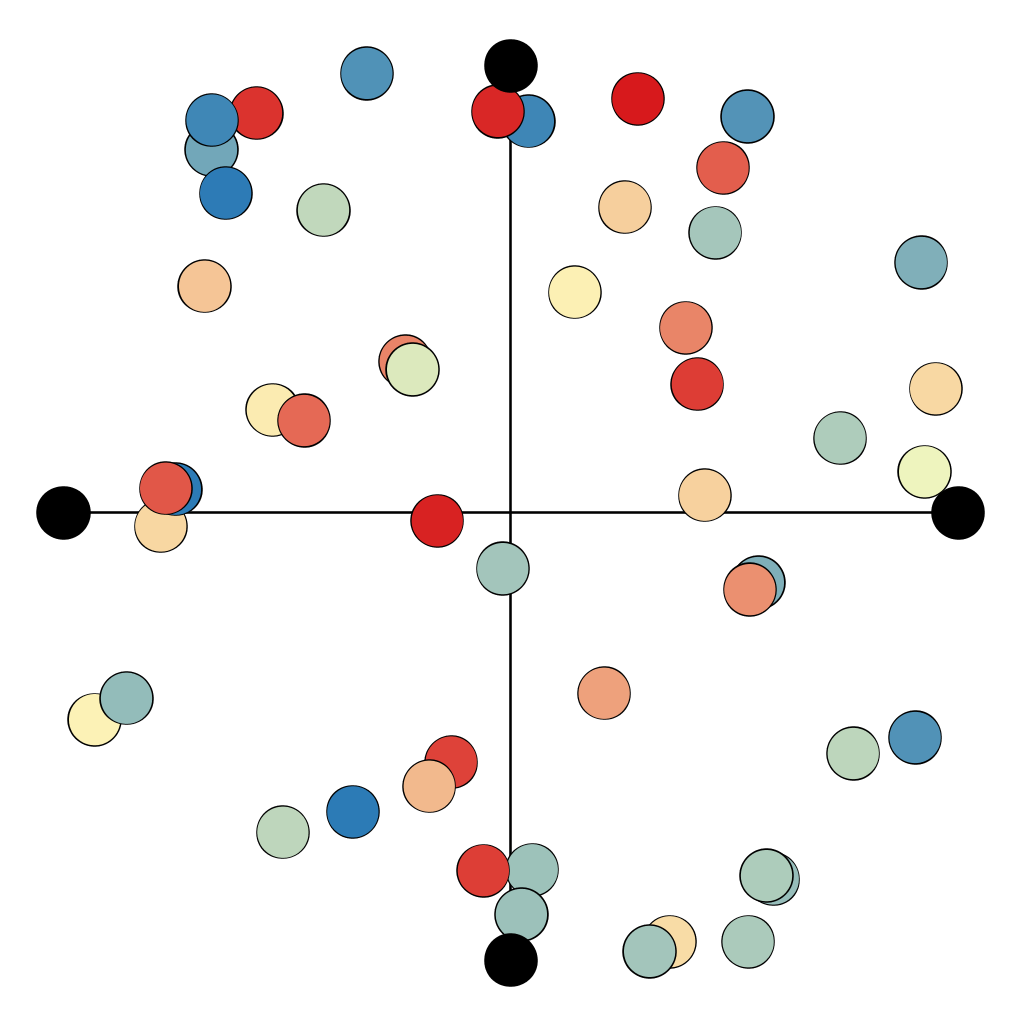
\includegraphics[width=\linewidth]{images/Evolutions/WB_0.png}
  \captionof*{figure}{Step 0}
\endminipage\hfill
\minipage{0.24\textwidth}
\centering
  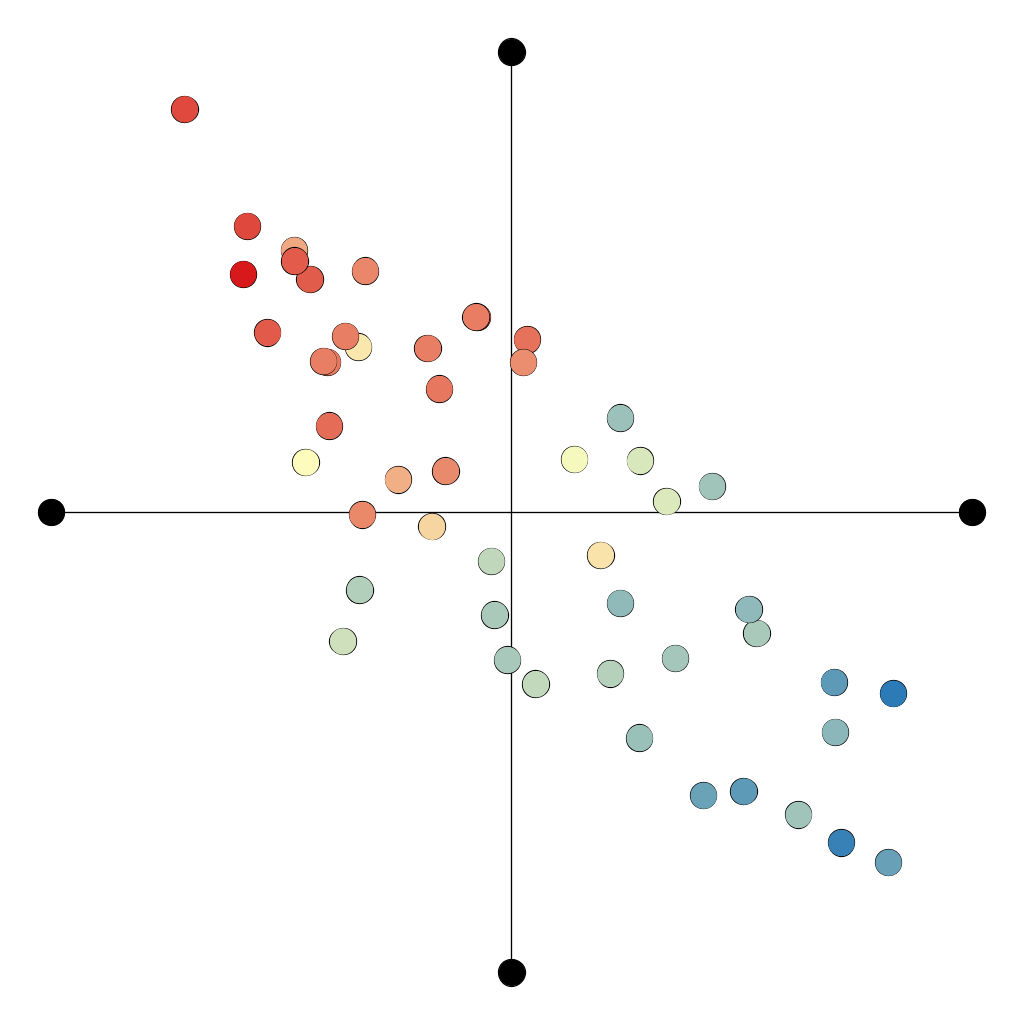
\includegraphics[width=\linewidth]{images/Evolutions/WB_0300_02.png}
  \caption*{Step 300}
\endminipage\hfill
\minipage{0.24\textwidth}
  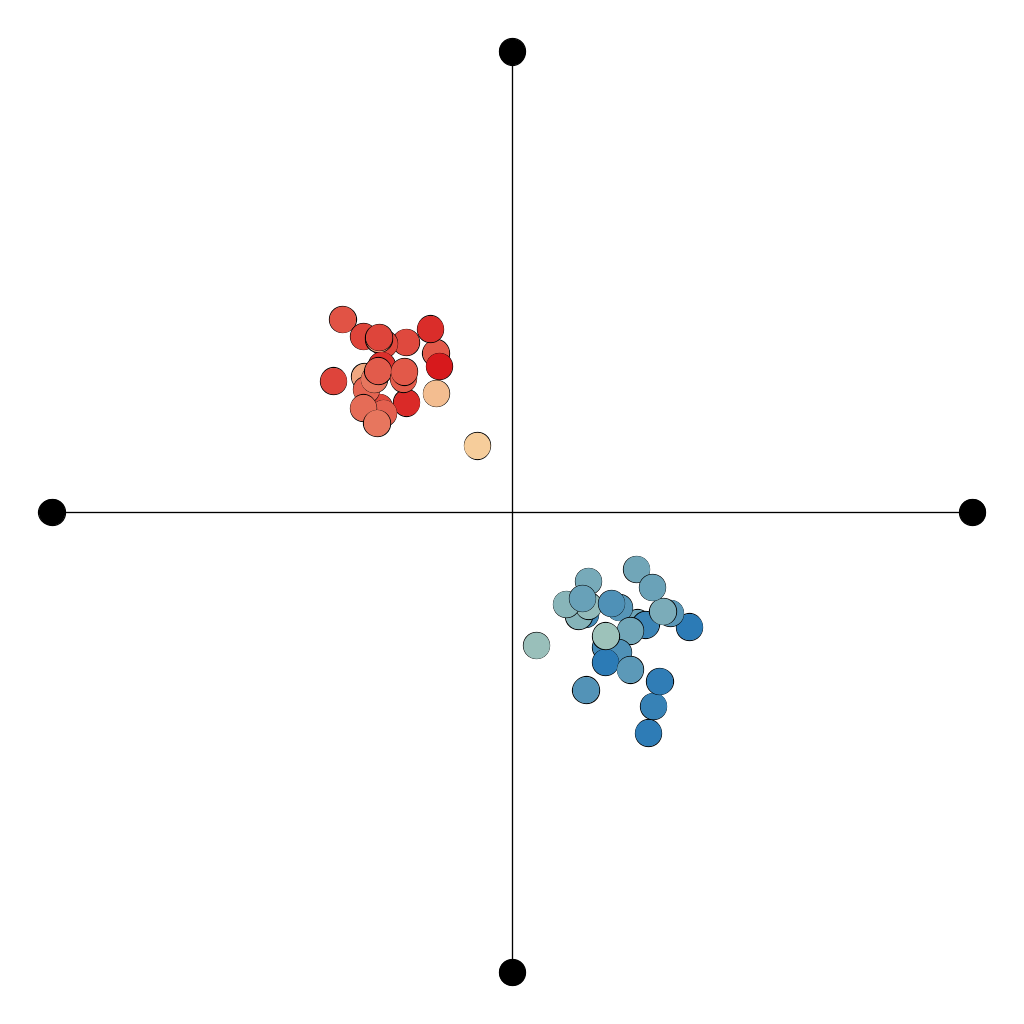
\includegraphics[width=\linewidth]{images/Evolutions/WB_0600_02.png}
  \caption*{Step 600}
\endminipage\hfill
\minipage{0.24\textwidth}
  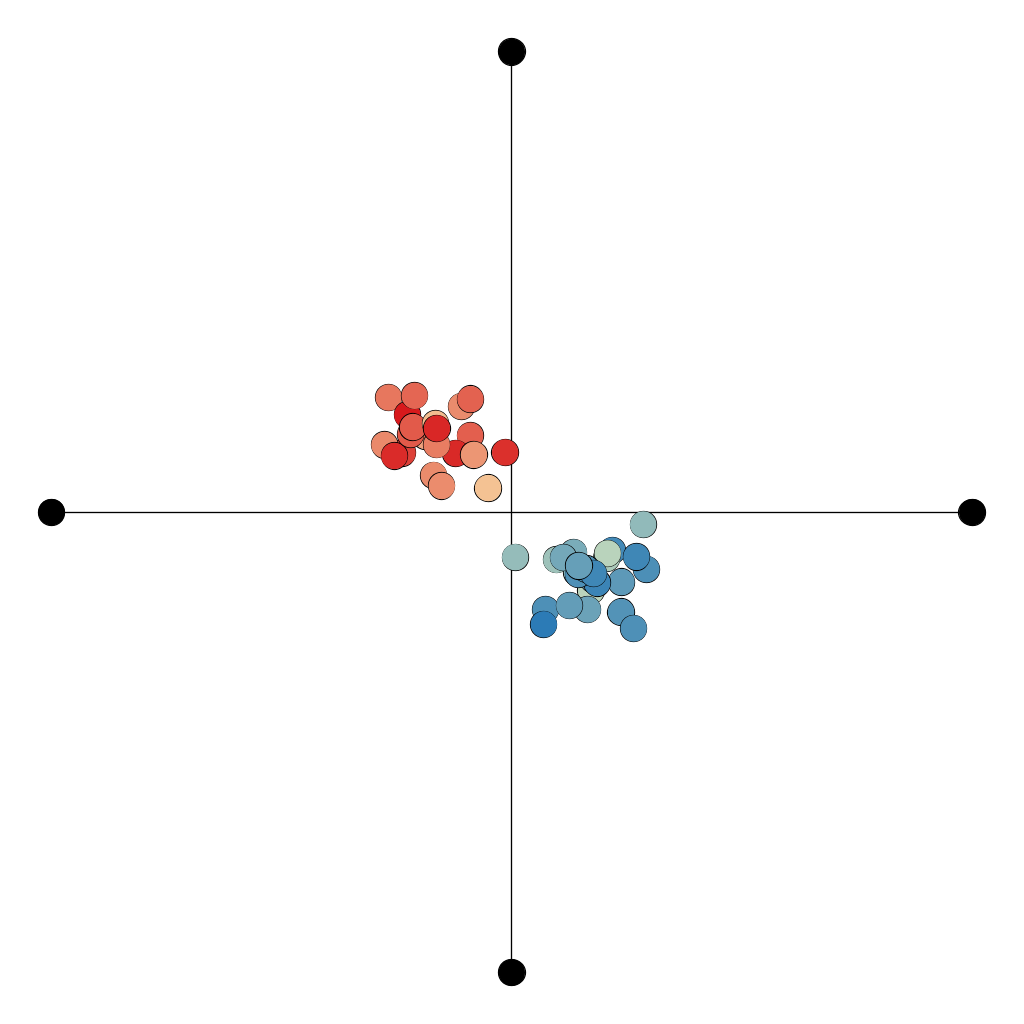
\includegraphics[width=\linewidth]{images/Evolutions/WB_3000_02.png}
  \caption*{Step 3000}
\endminipage\hfill
\vspace{0.5cm}
\caption{Various Steps of the Weighted Balance Model with 50 nodes and in a complete graph.Further f(x)=x (i.e. e=0). The x and y axis represent one opinion each, while coloring represents the third opinion. Black nodes are opinion extremes with values of +/-1 for the first image. Second, third and fourth image have black coordinates of value +/-0.2. Edges are not drawn.}
\label{WBT_Evo}
\end{figure}



These observations lead to the conclusion that the configuration of the basic WBT model at convergence is constrained to a set of the size of half the number of vertices in a hypercube, i.e. $2^D/2$. These final states are always composed of opposite clusters of agents with opposing opinion vectors. The model does not allow for 'moderate' nor more uniformly distributed states and is thus quite limited in its behavior.

\subsection{Generalized Weighted Balance Model}
For the general model, we embedded the WBT model into a network similar to the coevolution model but with multiple opinion dimensions. The defining feature characterizing the behavior in this model lies in the form of the $\text{connect}$-function. While we tested several functional forms, e.g. one based on the angle or matching signs of the opinions, we ultimately decided to use a criterion based on the euclidean distance between two agents' opinion vectors:
\[
\text{connect}( \mathbf{o}(i), \textbf{o}(j)) = 
 \begin{cases} 1 &\mbox{if } |  \mathbf{o}(i) - \textbf{o}(j)| < \varepsilon(N,D,z) \\
0 & \mbox{else } \end{cases}
\]
This approach relates to the sociological observation that people tend to form connections with those that do not stray too far from their own opinions (\citet{bahns2017similarity}) and often form echo chambers that further fortify their stances.  

In order to reduce complexity, we decided to focus on the role of the probability to form a new connection $\phi$ and the distance parameter $\varepsilon$ which indicates a node's "sphere of influence", to nodes in which it can connect. We find distinctly different behavior depending on the choice of these parameters as can be seen in the contour plot of the maximum (non-overlapping) component size $S$ (figure \ref{wbt_cont}). 


\begin{figure}[!htb]
    \centering
    \subfigure[$M=500$]{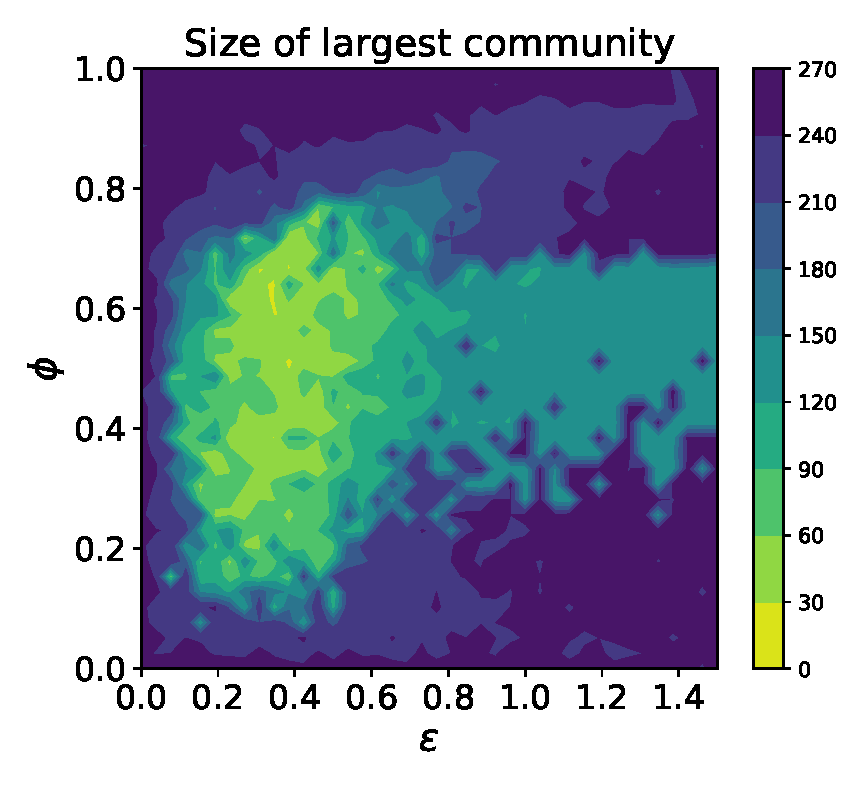
\includegraphics[width=0.47\textwidth]{images/WBT_general/contour_WBT_new.pdf}}
     \subfigure[$M=1000$ (color bar with different scale)]{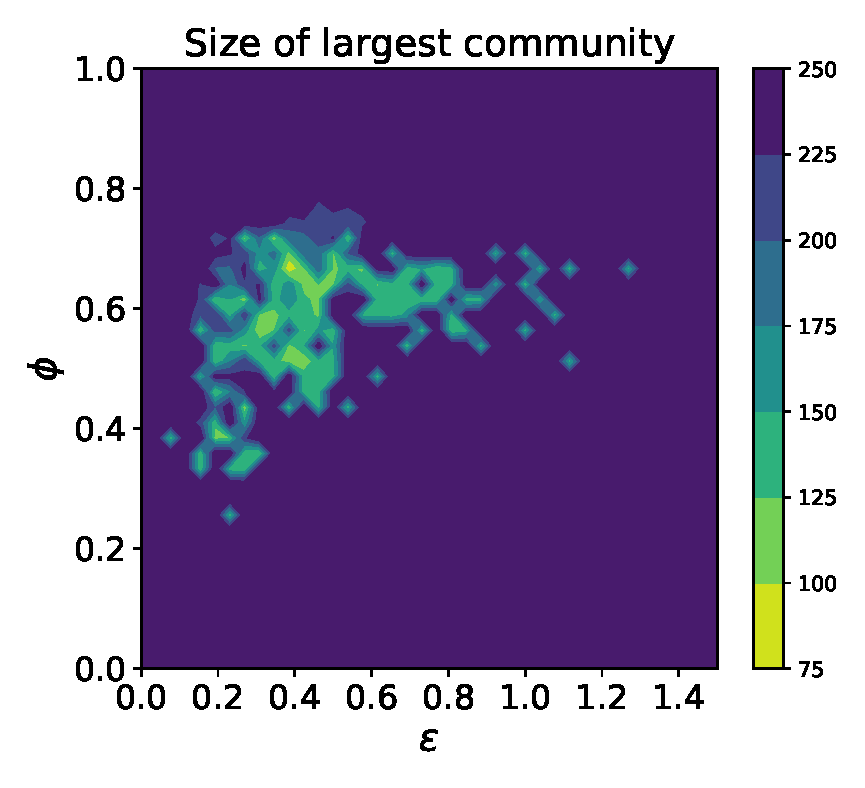
\includegraphics[width=0.47\textwidth]{images/WBT_general/contour_WBT_D1000_new.pdf}}
    \caption{Contour plot for WBT general $S(\varepsilon,\phi)$. $N=250$, $D=5$, $e=0.4$, $z=0.01$, $\alpha=0.3$. With $S \simeq N/2$ the system exhibits splitting into two similarly sized communities (cf. Figure \ref{WBT_g2}), which is not apparent from this contour plot. With increasing number of edges, the network exhibits less phases leading to mostly uniform alignment except for a small region.}
    \label{wbt_cont}
\end{figure}

Next, we looked at the network evolution of particular set of parameters which can be seen in Figures \ref{WBT_g2} (splitting into two main clusters) and Figure \ref{WBT_gm} (fragmentation into several clusters). There, the graphs are qualitatively depicted with their vertices and edges, however the opinions are not apparent in this visualization. For this, we reduced the model to two and three opinion dimensions, which will be discussed later (cf. Figure \ref{general_evo}). 



\begin{figure}[htb!]
  \centering
   \begin{tabular}{@{}p{0.33\linewidth}@{\quad}p{0.33\linewidth}@{\quad}p{0.33\linewidth}@{}}
    \subfigimg[width=\linewidth]{$t=0$}{images/WBT_general/testN250D500phi05eps1/0.png} &
    \subfigimg[width=\linewidth]{$t=17500$}{images/WBT_general/testN250D500phi05eps1/17500.png} &
    \subfigimg[width=\linewidth]{$t=30000$}{images/WBT_general/testN250D500phi05eps1/30000.png}
  \end{tabular}
  \caption{Exemplary convergent model run for $N=250$, $M=500$, $|D|=5$, $\varepsilon =1$, $\phi=0.5$, $z=0.01$, $\alpha=0.4$, $S=129$. The model displays gradual splitting into  two larger hyperpolarized communities as well as some singular nodes. This outcome corresponds to the outcome of the simpler WBT model. Note that the timesteps correspond to a single update for a node contrary to an update on the all nodes as previously defined.}
  \label{WBT_g2}
\end{figure}

\begin{figure}[htb!]
  \centering
  \begin{tabular}{@{}p{0.33\linewidth}@{\quad}p{0.33\linewidth}@{\quad}p{0.33\linewidth}@{}}
    \subfigimg[width=\linewidth]{$t=0$}{images/WBT_general/testN250D500phi05eps06/0.png} &
    \subfigimg[width=\linewidth]{$t=7500$}{images/WBT_general/testN250D500phi05eps06/7500.png} &
    \subfigimg[width=\linewidth]{$t=30000$}{images/WBT_general/testN250D500phi05eps06/30000.png}
  \end{tabular}
  \caption{Exemplary convergent model run with $N=250$, $M=500$, $|D|=5$, $\varepsilon =0.6$, $\phi=0.5$, $z=0.01$, $\alpha=0.4$ and $S=62$. The model displays gradual splitting into  6 larger communities as well as some very small and singular ones. Note that the timesteps correspond to a single update for a node contrary to an update on the all nodes as previously defined.}
  \label{WBT_gm}
\end{figure}


We compared the general model with the WBT model and found that with the parameters chosen, the opinions converge again to the corners of the opinion space, but conversely to WBT, they occupy many or all corners, as can be seen in Figure \ref{general_evo}. We therefore have a high polarisation for the individual opinions but less hyperpolarization as defined in the metric $H(O)$ within the model proposed by Schweighofer et al; individuals have extreme opinions, but the different opinions are distributed more dispersedly. There also remain a few unconnected nodes that are too far apart from other nodes to reconnect and therefore do not change their opinion. 

\begin{figure}[!htb]
  \centering
 \begin{tabular}{@{}p{0.33\linewidth}@{\quad}p{0.33\linewidth}@{\quad}p{0.33\linewidth}@{}}
    \subfigimg[width=\linewidth]{}{images/WBT_general//general_evo_1.pdf} &
    \subfigimg[width=\linewidth]{}{images/WBT_general/general_evo_2.pdf} &
    \subfigimg[width=\linewidth]{}{images/WBT_general/general_evo_4.pdf} 
    
  \end{tabular}
  
  \caption{Generalized Model with randomly initialized dynamic graph, $N=250$, $N_{edges}=500$, $D=3$, $e=0.3$, $\alpha = 0.3$, $\phi = 0.45$, $\varepsilon(N,D,z)=0.3$. The opinions converge in the corners. We can see opinion fragmentation but not hyperpolarization.}
  \label{general_evo}
\end{figure}

Moreover, looking at the network structure evolution in Figure \ref{dynamic graph} we see that the edges between communities vanish when they move apart in the opinion space. Our extension to the WBT model shows that when taking into account the evolving network structure within a population, opinions do not necessarily converge to a previously observed hyperpolarized state \footnote{However, fine-tuning the parameters (cf. Figure \ref{WBT_g2}) can still lead to analogous results.}.

\begin{figure}[h!]
\minipage{0.24\textwidth}
  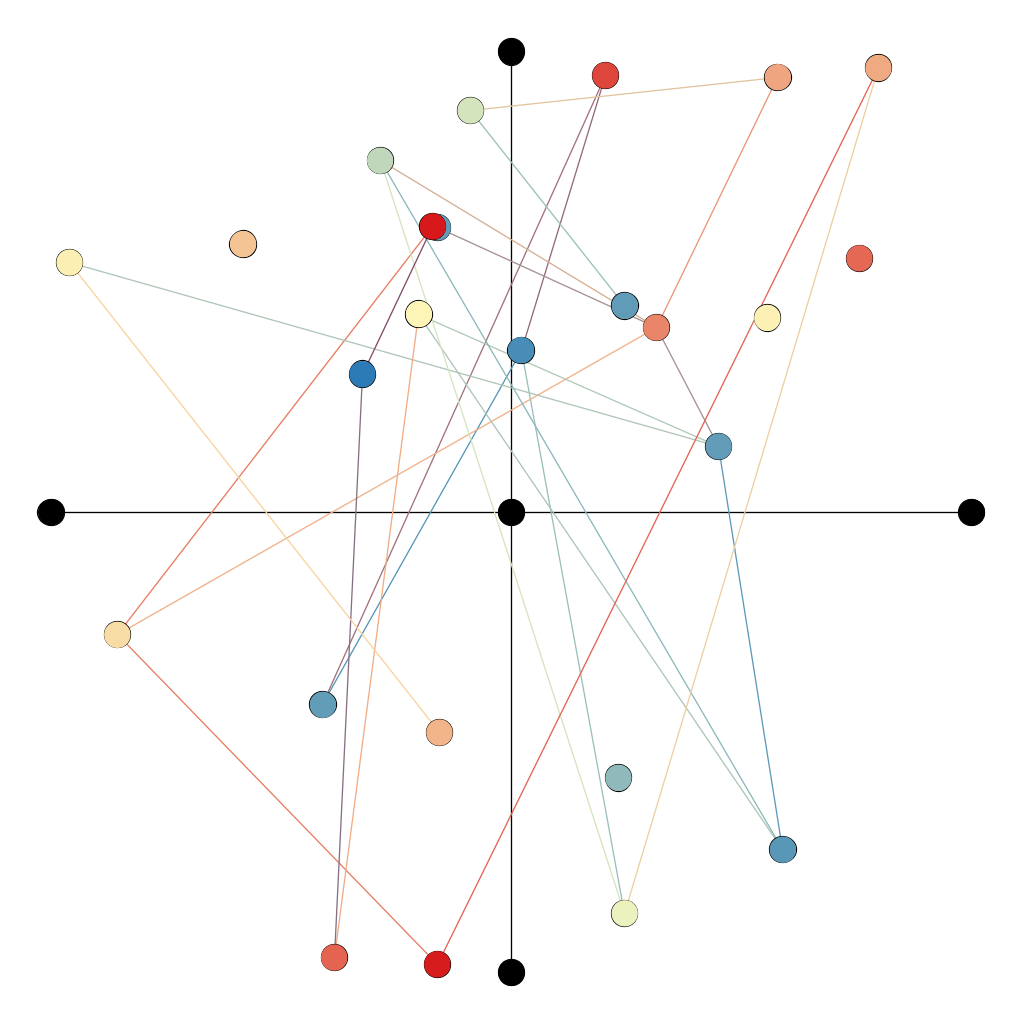
\includegraphics[width=\linewidth]{images/Evolutions/WBG25_0.png}
  \captionof*{figure}{Step 0}
\endminipage\hfill
\minipage{0.24\textwidth}
\centering
  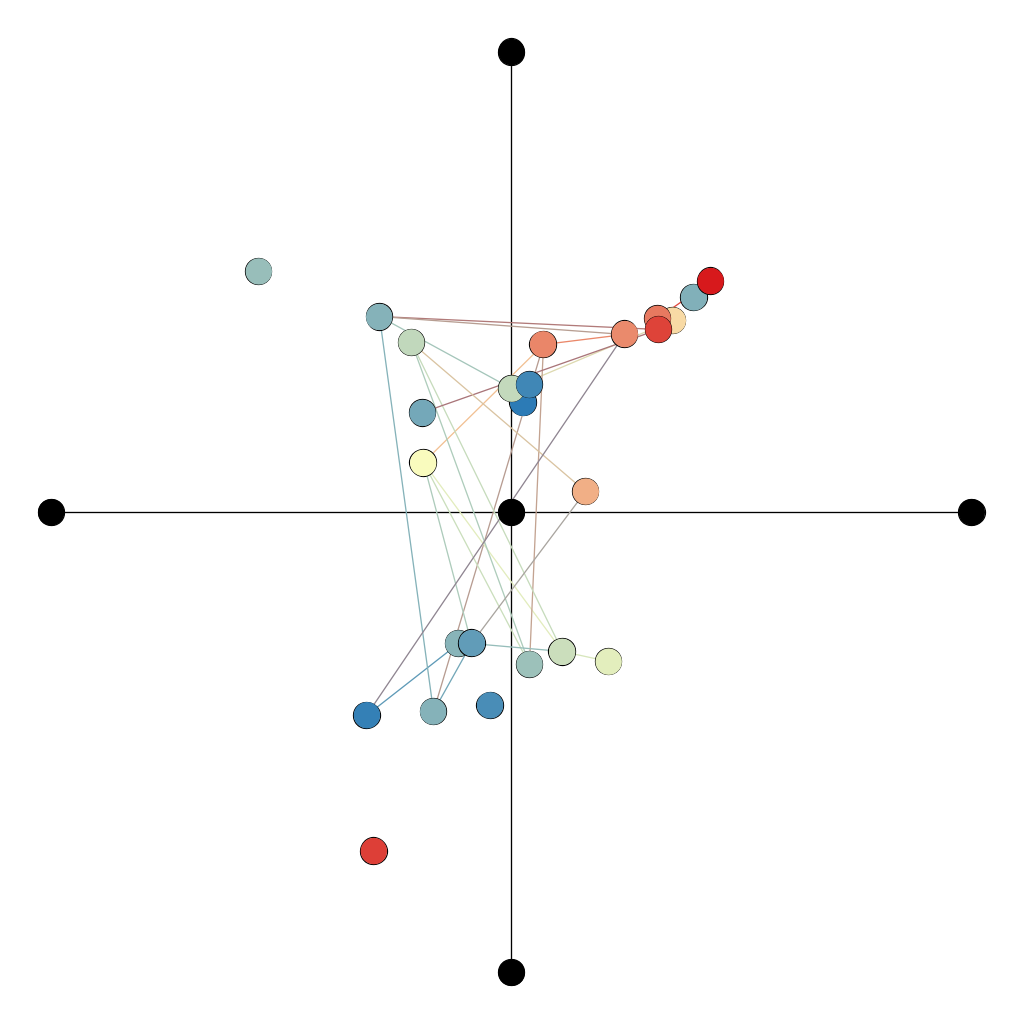
\includegraphics[width=\linewidth]{images/Evolutions/WBG25_300.png}
  \caption*{Step 300}
\endminipage\hfill
\minipage{0.24\textwidth}
  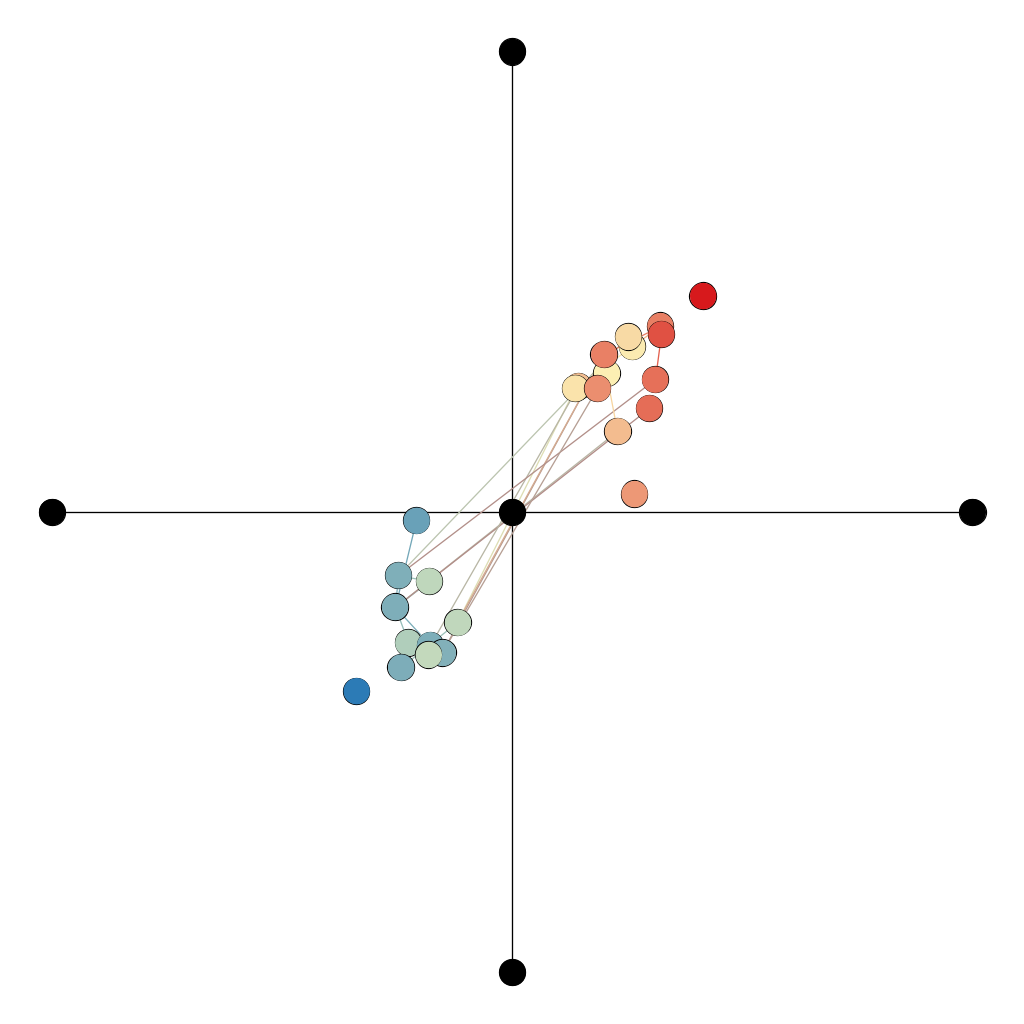
\includegraphics[width=\linewidth]{images/Evolutions/WBG25_600.png}
  \caption*{Step 600}
\endminipage\hfill
\minipage{0.24\textwidth}
  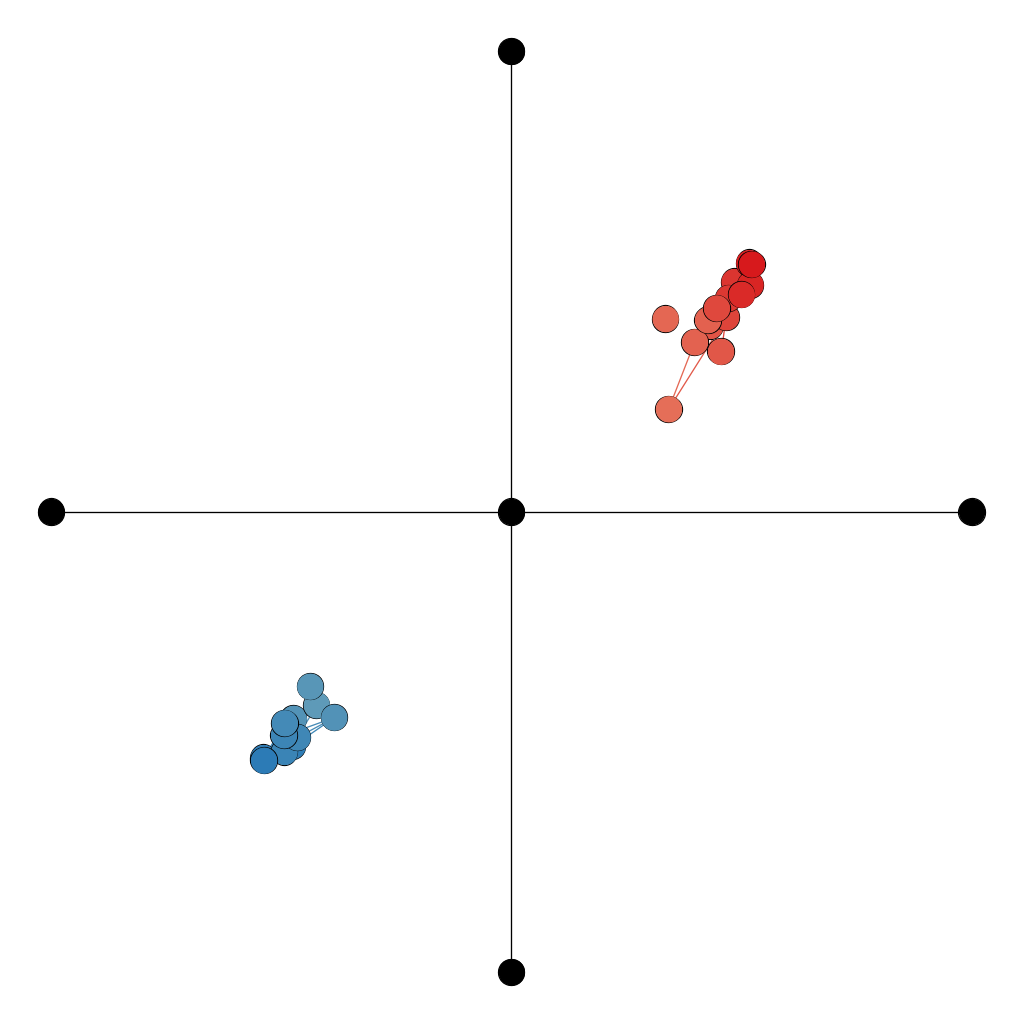
\includegraphics[width=\linewidth]{images/Evolutions/WBG25_1000.png}
  \caption*{Step 1000}
\endminipage\hfill
\caption{Various Steps of the General Model with 25 nodes and 25 edges, maximal connection distance is 1. The x and y axis represent one opinion each, while coloring represents the third opinion. Black nodes are coordinate extremes with values of +/-1 and the center.}
\label{dynamic graph}
\end{figure}


In contrast to the previous WBT model, our generalized model shows a myriad of varying behaviours. The model is far less constrained, however, the number of parameters makes systematic description difficult. Within this section we showed that both classical hyperpolarization as well as fragmentation into similarly sized communities are possible. 
\FloatBarrier
\subsection{Bots}
\subsubsection{Fully connected graph}
Adding bots that promote extreme opinions to the basic WBT model (fully connected and static graph) can lead to hyperpolarization even without evaluative extremeness, which is illustrated in Figure \ref{bots}. While near-maximal hyperpolarization happens even without bots for positive values of the evaluative extremeness parameter $e$, hyperpolarization is low without bots but increases rapidly as bots are added for $e=0$. 
\begin{figure}[!h]
\begin{center}
\subfigure[Bots with $o=1$ for all dimensions.]{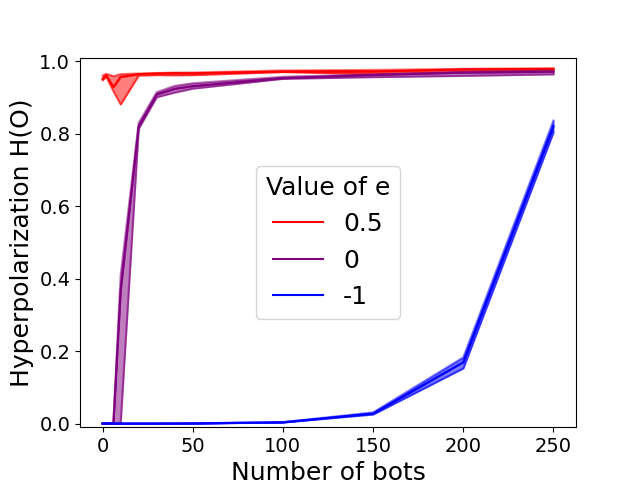
\includegraphics[width=0.49\textwidth]{images/Bots/H_bots.png}}
\subfigure[Half of bots with $o=1$ and the half with $o=-1$ for all dimensions. ]{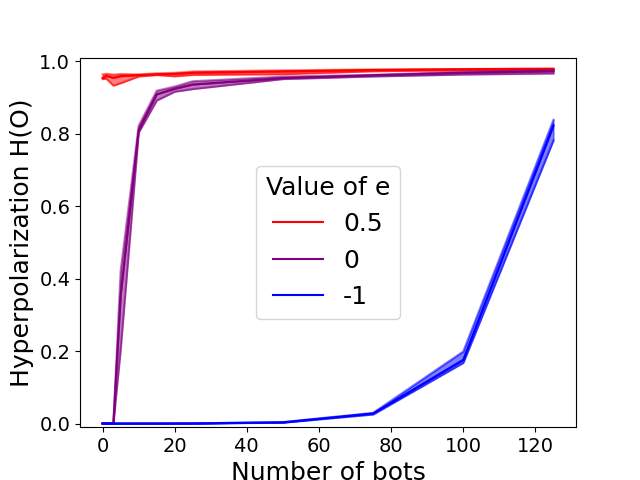
\includegraphics[width=0.49\textwidth]{images/Bots/H_bots_double.png}}
\end{center}
\caption{Hyperpolarization at convergence/after 100k single updates for Weighted Balance on a fully connected graph, $N=500$, $D=3$, $\alpha=0.4$, $z=0.01$, $f(x)=\sign(x)\cdot|x|^{1-e}$. Area between $10\%$- and $90\%$- empirical quantile over 10 runs shaded. Bots excluded from the calculation of H.}
\label{bots}
\end{figure}
Hyperpolarization also increases with the number of bots for negative evaluative extremeness $e$, but maximal hyperpolarization is not reached, even when half of the population consists of bots. Notably, there is no difference between having an equal number of bots on both extremes or having twice the amount of bots on a single side. This is because 
\[\text{SGM}(\textbf{o}(i),-\textbf{o}(j))=-\text{SGM}(\textbf{o}(i),\textbf{o}(j))=\text{SGM}(-\textbf{o}(i),\textbf{o}(j)),\] which implies \begin{align*}
A_{ij}&=f\left(\frac{1}{D}\sum_{d=1}^{D}\text{SGM}(o_{d}(i),o(j)))\right) =-f\left(\frac{1}{D}\sum_{d=1}^{D}\text{SGM}(o_{d}(i),-o(j)))\right)=A'_{ij},
\end{align*} for uneven $f$ with $f(-x)=-f(x)$, where $A'_{ij}$ is the value of $A_{ij}$ if the opinion of node $j$ was flipped. But in the absence of noise, the Weighted Balance update just moves $\textbf{o}(i)$ in the direction of \[
\text{SGM}(A_{ij},\mathbf{o}(j))=\text{SGM}(-A_{ij},-\mathbf{o}(j))=\text{SGM}(A_{ij}',-\mathbf{o}(j)),
\] 
implying that the update of node $i$'s opinion is never affected by flipping the counterparts' opinion as long as $f$ is uneven as we use the functional form $f(x)=\sign(x)\cdot|x|^{1-e}$. This symmetry might also explain why the mean opinion is essentially unaffected by the bots as can be seen in Figure \ref{bots_mean}. However, it is worth noting that the effect of bots on hyperpolarization diminishes, while the effect on the mean grows if non-bot opinions are initialized with nonzero expectation rather than uniformly from $[-1,1]^d$, as can be seen in Figure \ref{bots_shifted}.
\FloatBarrier
\subsubsection{Static graphs}
Moving from fully connected to more sparse static graphs has three effects that can be seen in  Figure \ref{bots sparse}: First, between-run variability for the same parameters is increased as the graph is initialized randomly. Second, hyperpolarization is smaller for uniformly randomly sampled edges compared to Barabási–Albert graphs, likely because of isolated nodes that remain unaffected by their surroundings. Third, the relative impact of the number of bots on hyperpolarization is lower than in the fully connected case, except for small numbers of bots and negative evaluative extremeness $e$. \begin{figure}[!h]

\subfigure[Edges sample uniformly ]{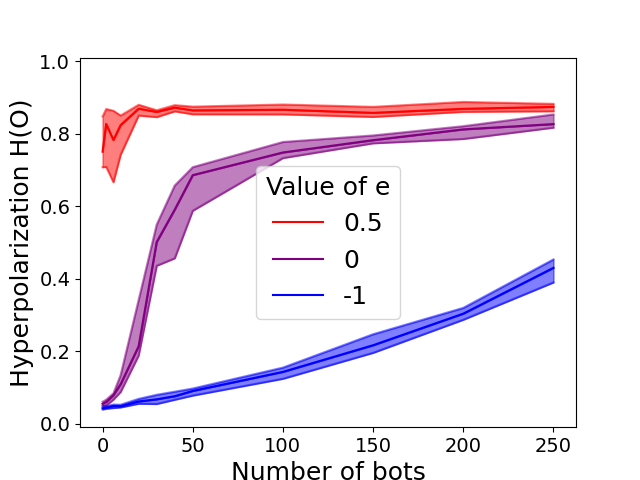
\includegraphics[width=0.49\textwidth]{images/Bots/H_bots_edges_500.png}}
\subfigure[Edges sampled accoruding to Barabási–Albert model]{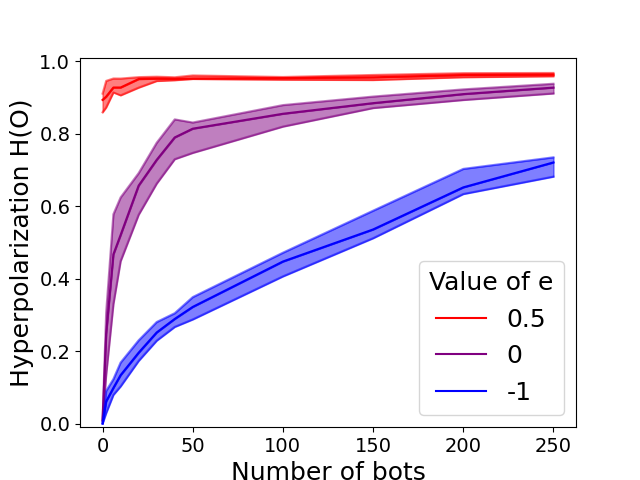
\includegraphics[width=0.49\textwidth]{images/Bots/H_bots_ba___edges_499.png}}

\caption{Hyperpolarization at convergence/after 100k single updates for Weighted Balance, static graph with $499$ edges, $N=500$, $D=3$, $\alpha=0.4$, $z=0.01$, $f(x)=\sign(x)\cdot|x|^{1-e}$ and varying amount of bots with $o=1$ for all dimensions. Area between $10\%$- and $90\%$- empirical quantile over 10 runs shaded.}
\label{bots sparse}
\end{figure}
Next, Figure \ref{bots ba bt} shows the effect of the bots' centrality on hyperpolarization: perhaps unsurprisingly, placing bots in the most connected nodes of an exponential Barabási–Albert graph magnifies their effect, while placing them in the least central nodes makes them a lot less effective. 
\begin{figure}[h!]
\subfigure[Bots placed in the most connected nodes.  ]{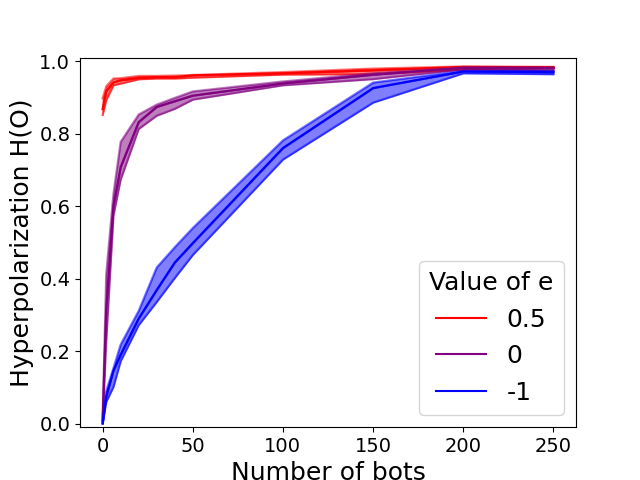
\includegraphics[width=0.49\textwidth]{images/Bots/H_bots_ba_top__edges_499.png}}
\subfigure[Bots placed in in the least connected nodes. ]{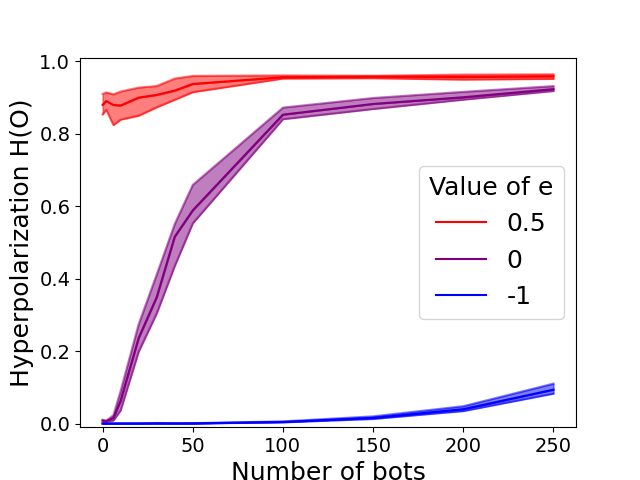
\includegraphics[width=0.49\textwidth]{images/Bots/H_bots_ba_bottom__edges_499.png}}
\caption{Hyperpolarization at convergence/after 100k single updates for Weighted Balance with randomly intialized Barabási–Albert graph with $499$ edges, $N=500$, $D=3$, $\alpha=0.4$, $z=0.01$, $f(x)=\sign(x)\cdot|x|^{1-e}$ and varying amount of bots with $o=1$ for all dimensions. Area between $10\%$- and $90\%$- empirical quantile over 10 runs shaded. Bots excluded from the calculation of H.}
\label{bots ba bt}
\end{figure}

Adding bots that spread neutral opinions reduces hyperpolarization, as can be seen for $e=0.5$ in Figure \ref{bots neutral ba bt}. However, a large number of such bots can be necessary to combat evaluative extremeness, especially if the bots are placed in noncentral nodes. 

\begin{figure}[h!]
\subfigure[Neutral bots with $o=0$ for all dimensions placed in the most connected nodes.]{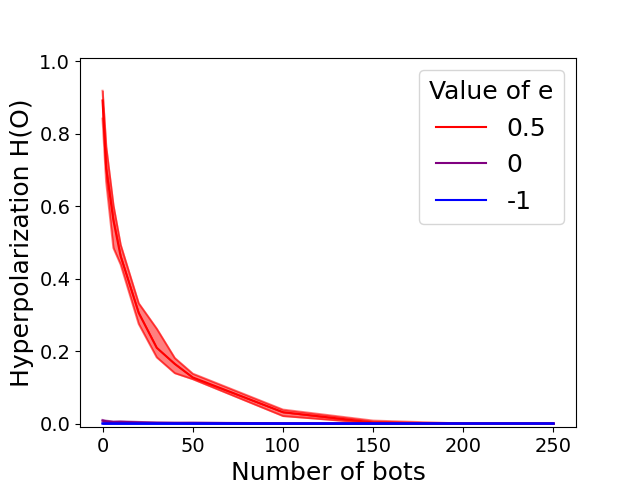
\includegraphics[width=0.49\textwidth]{images/Bots/H_bots_ba_top__neutral_edges_499.png}}
\subfigure[Neutral bots with $o=0$ for all dimensions placed in the least connected nodes.]{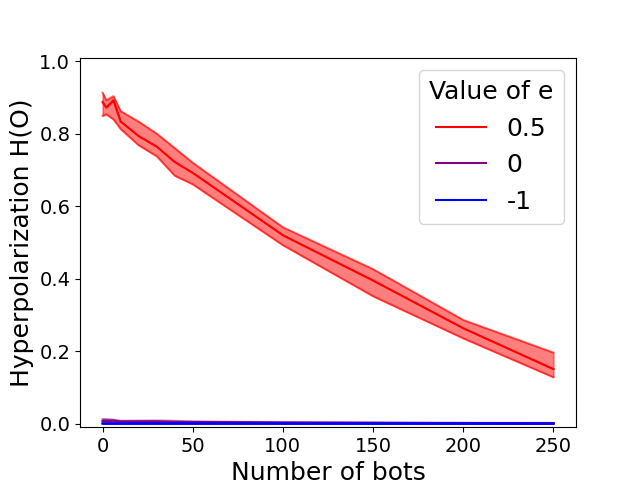
\includegraphics[width=0.49\textwidth]{images/Bots/H_bots_ba_bottom__neutral_edges_499.png}}
\caption{Hyperpolarization at convergence/after 100k single updates for Weighted Balance on static Barabási–Albert graph with $499$ edges,  $N=500$, $D=3$, $\alpha=0.4$, $z=0.01$, $f(x)=\sign(x)\cdot|x|^{1-e}$. Area between $10\%$- and $90\%$- empirical quantile over 10 runs shaded. Bots excluded from the calculation of H.}
\label{bots neutral ba bt}
\end{figure}

As can be seen in \ref{bots altf}, breaking the symmetry in $f$ can cause a range of interesting behaviour. When only attractive or repulsive forces are considered ($f$ equal to the minimum or maximum of $x$ and $0$), the average opinion for every dimension can be influenced by the bots, unlike in the previous cases. With attractive forces, it converges to the bots' opinion rather quickly, while repulsive forces cause slower convergence to the opposite opinion. Interestingly, the latter coincides with non-monotonous hyperpolarization if bots are placed in the most connected nodes: Without any bots, the repulsive forces mostly balance out such that the unpolarized initial configuration is mostly stable. Then, as bots are added, they cause nodes to take on the opposite extreme opinion, which in turn leads to other nodes being pushed towards the bots' opinion. As even more bots are added, this counteraction quickly weakens, as fewer and fewer connections between non-bot nodes remain.
Surprisingly, adding or subtracting a small constant to $f(x)=x$, representing a consistently biased opinion about other people increases hyperpolarization without bots regardless of the biases direction and has a rather small effect on the overall mean, independent of the direction in which the bias points. 
\begin{figure}[h!]
\subfigure[Hyperpolarization. ]{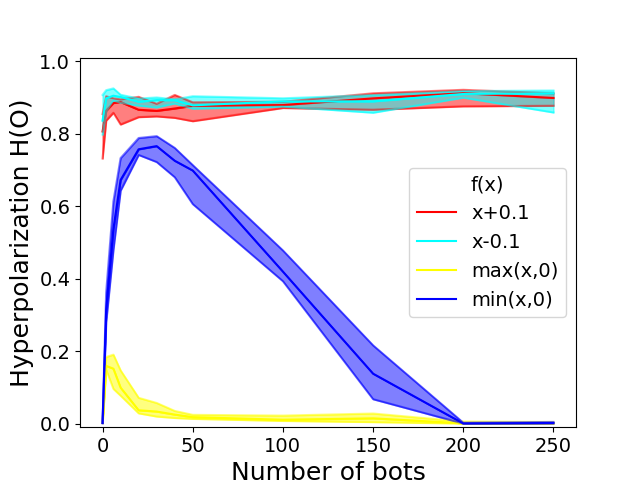
\includegraphics[width=0.49\textwidth]{images/Bots/H_bots_altf_ba_top_edges_499.png}}
\subfigure[Maximum (over dimensions) absolute mean opinion.]{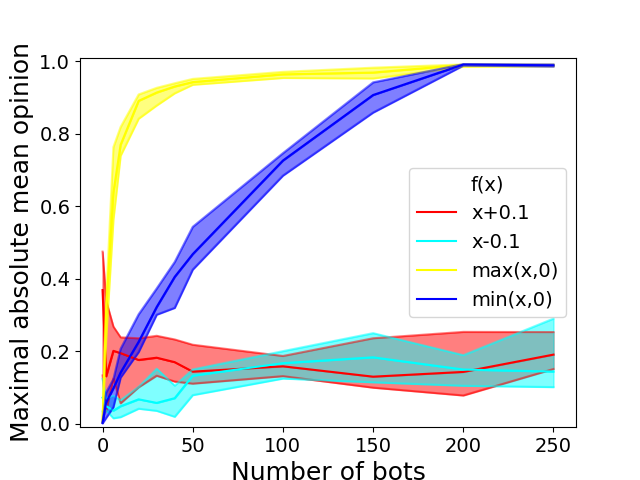
\includegraphics[width=0.49\textwidth]{images/Bots/maxabsop_bots_altf_ba_top_edges_499.png}}
\caption{Weighted Balance model on randomly initialized static Barabási–Albert graph with $499$ edges at convergence/after 100k single updates with $N=500$, $D=3$, $\alpha=0.4$, $z=0.01$ and varying amount of bots with $o=1$ for all dimensions. Bots placed in the most connected nodes. Area between $10\%$- and $90\%$- empirical quantile over 10 runs shaded. Bots excluded from the calculation of H and mean opinion.}
\label{bots altf}
\end{figure}
\FloatBarrier
\subsubsection{Dynamic graphs}
\begin{figure}[h!]
\subfigure[Bots use same connect function as other nodes]{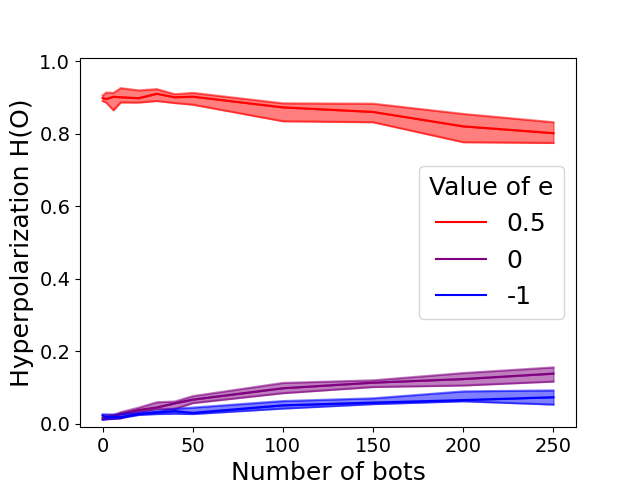
\includegraphics[width=0.49\textwidth]{images/Bots/H_bots_ba__edges_499_epsilon_10.png}}
\subfigure[Bots can connect to any node, not just close ones]{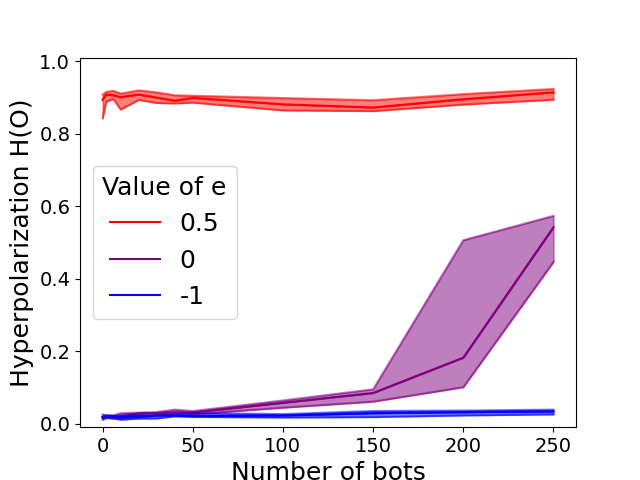
\includegraphics[width=0.49\textwidth]{images/Bots/H_bots_ba__seeking__edges_499_epsilon_10.png}}
\caption{Hyperpolarization in dynamic graph Weighted Balance model on randomly initialized Barabási–Albert graph with $499$ edges at convergence/after 100k single updates with $\phi=0.5$, distance-based connect function with $\varepsilon=1$ as well as $N=500$, $D=3$, $\alpha=0.4$, $z=0.01$. Varying amount of bots with $o=1$ for all dimensions. Area between $10\%$- and $90\%$- empirical quantile over 10 runs shaded. Bots excluded from the calculation of H.}
\label{bots dynamic}
\end{figure}

Adding bots to the Generalized WBT model for values of $\varepsilon$ and $\phi$ that led to moderate hyperpolarization in Figure \ref{wbt_cont} produces some interesting results. As can be seen in Figure \ref{bots dynamic}, the influence of bots on hyperpolarization is greatly diminished in dynamic graphs as the bots start with extreme opinions and thus quickly lose most of their connections to non-extreme nodes, even if the bots started out highly connected. Surprisingly, the bots influence is similarly small for moderate numbers of bots, when the connect function is modified such that bots sample their new connections from any node, not just close ones. Interestingly, the same effect can be seen when "competing" bots are placed in opposing corners of opinion space. However, the increase in hyperpolarization with large amount of bots is even more rapid but also more uncertain in that case, as can be seen in Figure \ref{bots dynamic_double}. 
\begin{figure}[h!]
\subfigure[No bots]{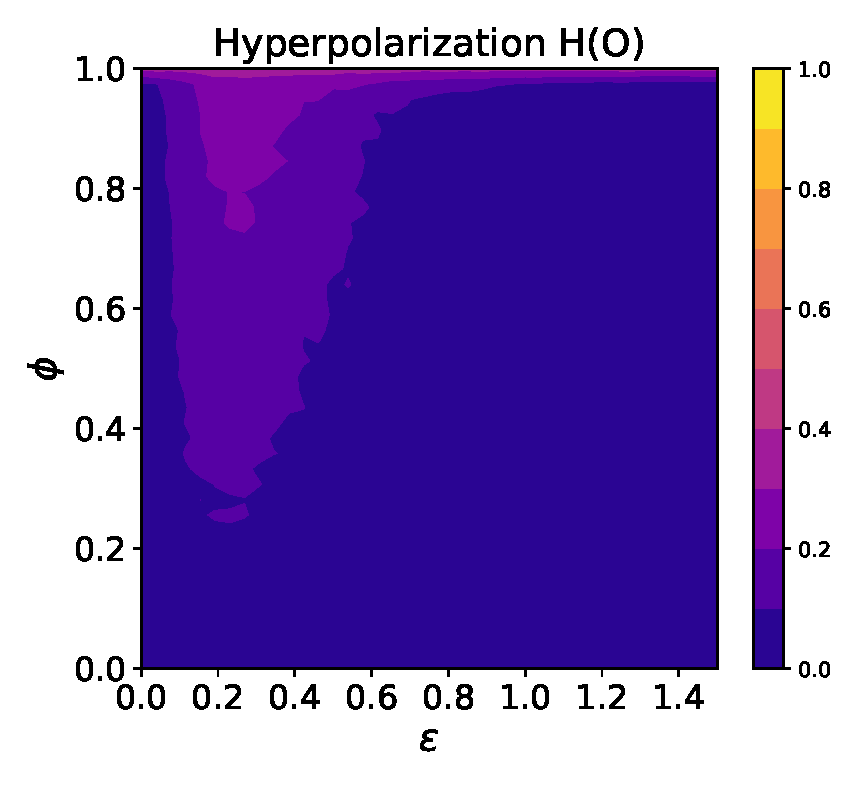
\includegraphics[width=0.32\textwidth]{images/Bots/contour_WBT_ba.pdf}}
\subfigure[50 bots constrained by $\varepsilon$]{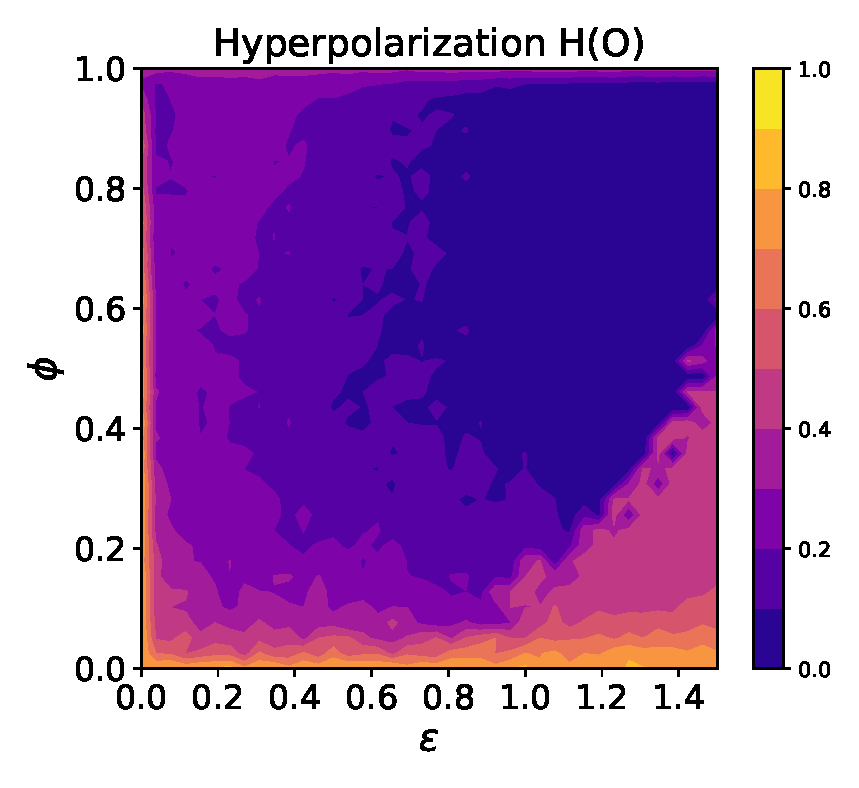
\includegraphics[width=0.32\textwidth]{images/Bots/contour_WBT_50bots_ba.pdf}}
\subfigure[50 bots unconstrained by $\varepsilon$ ]{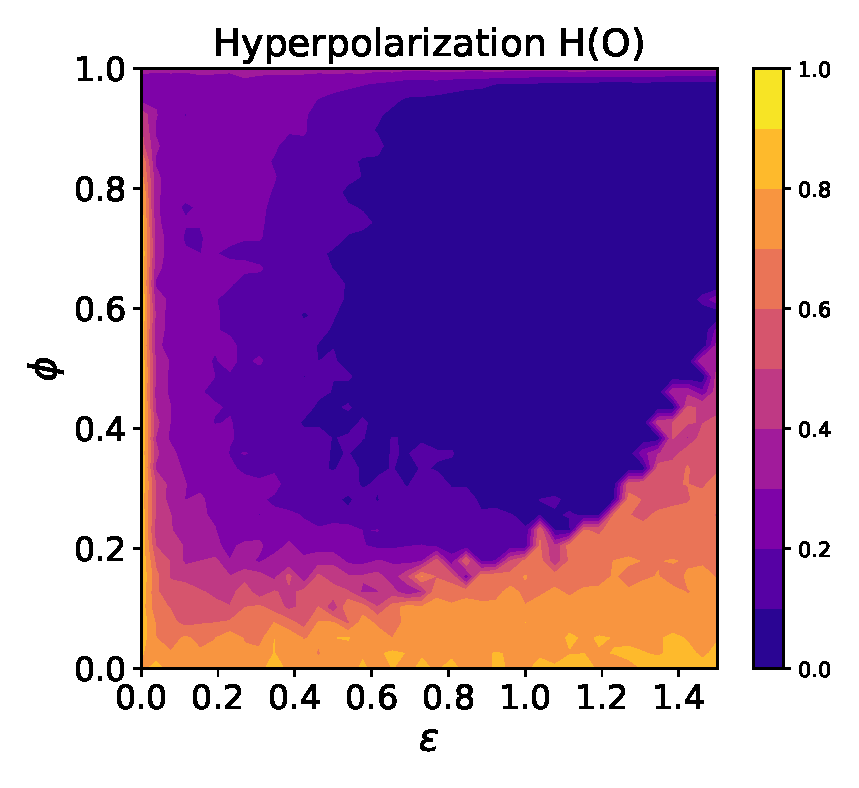
\includegraphics[width=0.32\textwidth]{images/Bots/contour_WBT_50bots_ba_seeking.pdf}}
\caption{Hyperpolarization for different levels of $\varepsilon$ and $\phi$ in  dynamic graph Weighted Balance model on Barabási–Albert graph with $499$ edges at convergence/after 100k single updates with $N=500$, $D=3$, $\alpha=0.4$, $z=0.01$. Bots with $o=1$ for all dimensions placed in random nodes and excluded from calculation of H. Bots have the strongest effect on hyperpolarization for small values of $phi$ and large values of $\varepsilon$. Similarly, the effect of allowing bots to connect to more distant nodes is most pronounced for these values. 
}
\label{bots contour}
\end{figure}
This might be because multiple updates are needed to bring a node close enough to the bots, such that it stays connected to them rather quickly replacing connections to bots by sampling its new connections exclusively from non-bots. To investigate this hypothesis, we looked at the hyperpolarization for different values of $\varepsilon$ and $\phi$ for $50$ (Figure \ref{bots contour}) and $200$ (Figure \ref{Bots contour 200}) bots sharing the same extreme opinion . There, allowing bots to connect to arbitrary nodes has the biggest effect for small values of $\phi$ and large values of $\varepsilon$. This fits our hypothesis as small values of $\phi$ mean that a node is less likely to update its connections after being connected to a bot. Similarly, for large $\varepsilon$, fewer updates are needed to get a node from outside the bots' sphere of influence to within the sphere, where it is less likely to disconnect from the bots. 

\begin{figure}[htb]
\subfigure[Bots connect in the same way as other nodes]{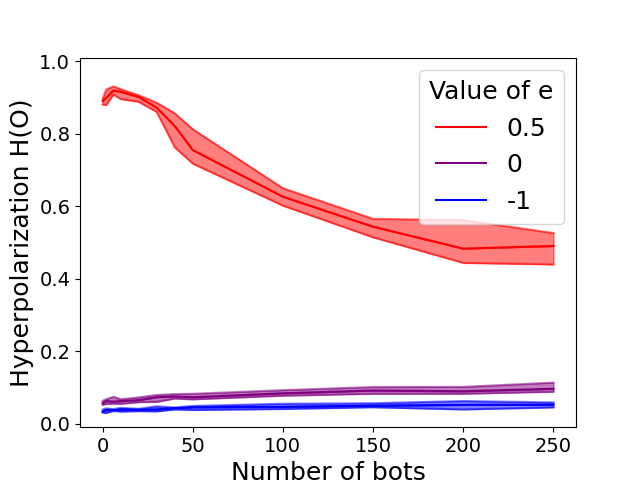
\includegraphics[width=0.49\textwidth]{images/Bots/H_bots_ba__neutral_edges_499_epsilon_6.png}}
\subfigure[Bots can connect to any node, not just close ones.  ]{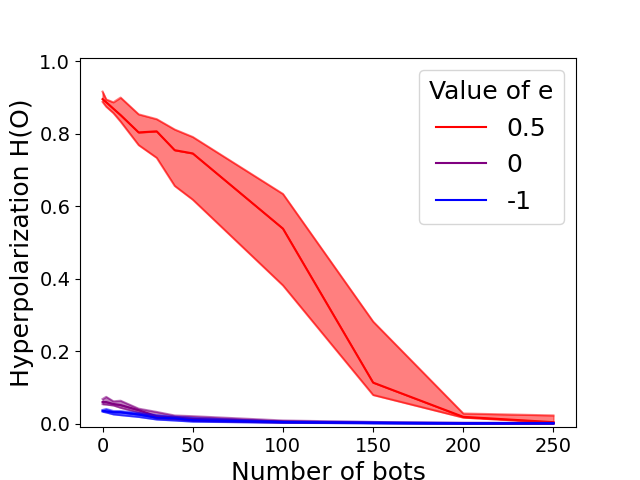
\includegraphics[width=0.49\textwidth]{images/Bots/H_bots_ba__seeking__neutral_edges_499_epsilon_6.png}}
\caption{Hyperpolarization in dynamic graph Weighted Balance model on randomly initialized Barabási–Albert graph with $499$ edges at convergence/after 100k single updates with $\phi=0.5$, distance-based connect function with $\varepsilon=0.6$, as well as $N=500$, $D=3$, $\alpha=0.4$, $z=0.01$. Area between $10\%$- and $90\%$- empirical quantile over 10 runs shaded. Varying amount of neutral bots with $o=0$ for all dimensions.Bots excluded from the calculation of H.}
\label{bots dynamic_neutral}
\end{figure}


The effect of neutral bots in the dynamic graph is more pronounced, but again small compared to static graphs (Figure \ref{bots dynamic_neutral}). Unlike with extreme bots, neutral bots with the ability to connect to arbitrary bots are able to reduce hyperpolarization to a similar extent as in a  static graph with bots placed in the least connected nodes. 

\begin{figure}[h] 
\subfigure[]{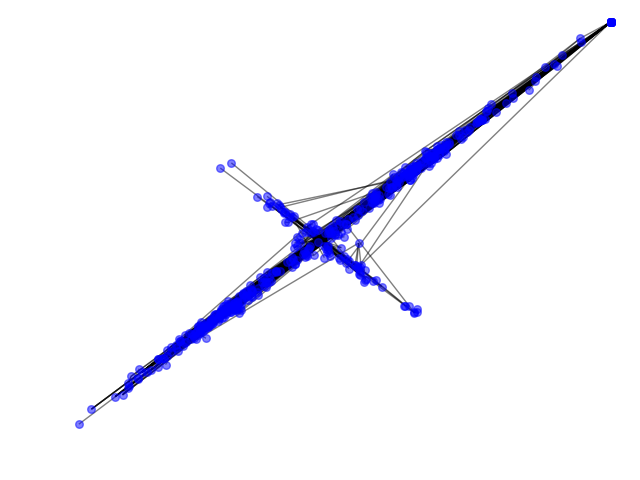
\includegraphics[width=0.19\textwidth,height=0.19\textwidth]{images/Bots/id_bots_edge_bottom24.png}}
\subfigure[]{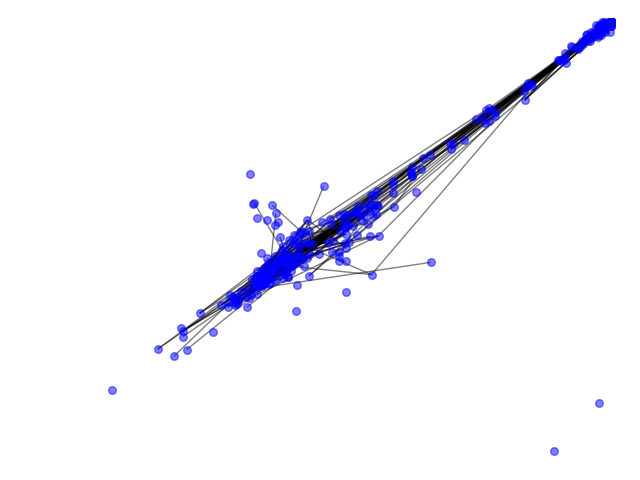
\includegraphics[width=0.19\textwidth,height=0.19\textwidth]{images/Bots/id_edge_top_eps1_200bots24.png}}
\subfigure[]{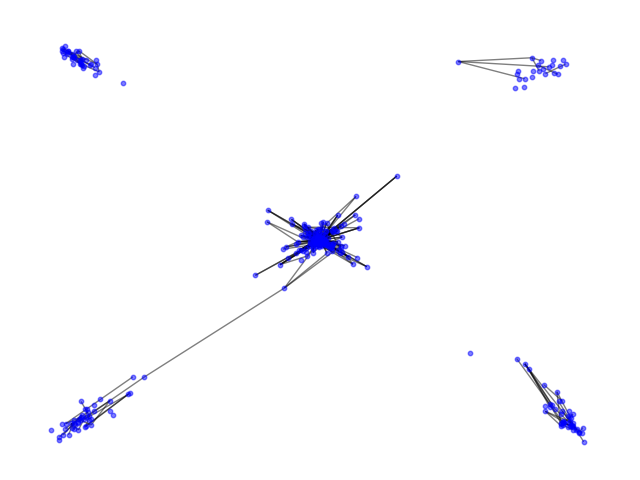
\includegraphics[width=0.19\textwidth,height=0.19\textwidth]{images/Bots/eval_extreme_edge_eps06_200neutral24.png}}
\subfigure[]{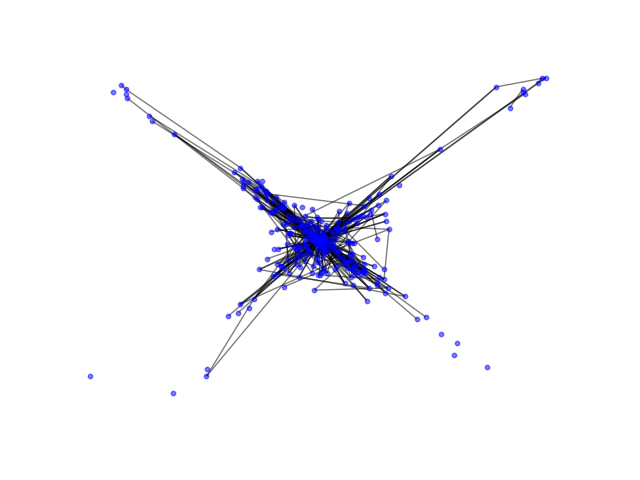
\includegraphics[width=0.19\textwidth,height=0.19\textwidth]{images/Bots/eval_extreme_edge_eps06_200neutral_seeking24.png}}
\subfigure[]{\includegraphics[width=0.19\textwidth,height=0.19\textwidth]{images/Bots/eval_extreme_edge_eps0624.png}}

\caption{Weighted Balance model on Barabási–Albert graph with $499$ edges after 25 steps per node with $N=500$, $D=2$, $\alpha=0.4$, $z=0.01$. a) Static graph, $e=0$, 50 bots ($o=1$) in least connected nodes. b) Dynamic graph ($\varepsilon=1,\phi=0.5$), $e=0$, 200 bots ($o=1$) in most connected nodes. c) Dynamic graph ($\varepsilon=0.6,\phi=0.5$), $e=0.5$, 200 neutral bots ($o=0$) in random nodes.
d) Dynamic graph ($\varepsilon=0.6,\phi=0.5$), $e=0.5$, 200 neutral bots ($o=0$) in random nodes. Bots unaffected by $\varepsilon$.
e) Dynamic graph ($\varepsilon=0.6,\phi=0.5$), $e=0.5$, no bots.
}
\label{samplemodels}
\end{figure}



 \clearpage
\section{Summary and Outlook} \label{sumandout}
We implemented, generalized and extended the opinion formation models by \citet{holme2006nonequilibrium} and \citet{schweighofer2020}.
During the reproduction of the coevolution model we saw very similar effects regarding the community sizes, as well as their phase transition, compared to the original paper.
Only minor deviations occurred, which we ascribe to our limitations in computational power resulting in simulations with smaller networks but qualitative findings were not influenced by this.
The reproduction of the Weighted Balance Theory model yielded the behaviour reported in the original paper, validating our implementation of the models.

The generalization and unification of the models let us combine the strengths of dynamic networks with attitude-based influence and thus allows us to account for previously neglected effects. 
The investigation of the effects of various parameters confirmed our theoretical suspicion that the evaluative extremeness parameter $e$ and more generally the choice of the attitude transformation \textit{f function} have a large impact on qualitative model behaviour and often determine the extent of hyperpolarization. Notably, hyperpolarization can also be affected by high levels of noise and is relevantly influenced by the choice of $\phi$ and $\varepsilon$ which specify the network behaviour in the dynamic model. 

With the inclusion of evolving networks, we were able to observe fragmentation into independent extreme opinions instead of hyperpolarization along a single axis when nodes prefer to connect to nodes that are very close to them in terms of opinion. This can be seen as an interesting starting point for the examination of effects of various connectivity configurations and shows that social media might not necessarily lead to the high hyperpolarization currently observed in the US: By leveraging the increased control over whom they connect to which is provided by social media, people can avoid societal polarization. However, it is not clear whether the resulting echo chambers and fragmentation are necessarily preferable from a societal point of view, especially if opinions still consistently increase in extremeness, as observed in the generalized WBT model with dynamic graphs. 

The impact of bots with fixed opinions on polarization varies but strongly depends on the evaluative extremeness and the connections bots start with and are able to maintain. In our simulations placing bots in the most connected nodes and letting them connect to a wider range of other nodes increased the effectiveness of bots, both polarizing and mediating ones. This is interesting as \citet{stella2018bots} came to the conclusion that social bots (in this case using tweets in twitter) mainly target human influencers on both sides of the opinion spectrum within a network, which can be interpreted as an attempt to leverage the influencers' connections to effectively influence many others' opinions. This is consistent with strategic behaviour that would be implied by extrapolating from our model. 

While our model in its current form is already able to provide a wide range of behaviour with different parameter choices (see figure \ref{samplemodels}), there is an abundance of possible extensions that could be performed. 
Firstly, the models do not consider factors like home city and hobbies which are important in the formation of real-life social networks, as well as the effect described by \citet{krosnick1990}, concerning interpersonal differences in the relative importance of certain topics and the extent to which they influence a person's attitude towards others. Also, historical data on political opinions and social network structures could be used to better understand which model parameters best describe real world opinion dynamics in different contexts. This might be especially important for the evaluative extremeness parameter, which has a huge impact on polarization produced by our model and has so far only been empirically investigated in the context of the highly polarized 2016 US presidential evaluation. More generally, an empirical investigation of the update dynamics specified by the Weighted Balance Theory model could be useful, as the model has some unintuitive properties: Apart from consistently producing extreme opinions for positive evaluative extremeness, even for isolated clusters of nodes with the same opinion, the model implies that people moderate their opinion when meeting somebody they feel neutral about. 
Next, the initialization of the model can affect its limiting behaviour and therefore, current trends might be better described with models initialized with pre-set biased opinions other than randomly distributed ones with mean zero.
Finally, expanding on our experiments with social bots, it could be interesting to see how their connecting strategy can be improved to maximize their effect on polarization in either direction. This could be done using simple heuristics, or more complex strategies that react to an evolving network, learnt by reinforcement learning. Similarly, further work could identify strategies society and individual citizens can employ to counter the influence of bots that do not come at the price of increased fragmentation. 

\bibliography{bibliography}
\bibliographystyle{plainnat}

\appendix
\section{Appendix}
\counterwithin{figure}{section}



\begin{figure}[!htb]
\begin{center}
\subfigure[Hyperpolarization: minimal initial opinion at -0.75 ]{\includegraphics[width=0.45\textwidth]{images/Bots/H_botsshifted_-75_100.png}}
\subfigure[Maximum (over dimensions) absolute mean opinion (graph as in a) ]{\includegraphics[width=0.45\textwidth]{images/Bots/maxabsop_botsshifted_-75_100.png}}\\[-2.3ex]
\subfigure[Hyperpolarization: minimal initial opinion at -0.5  ]{\includegraphics[width=0.45\textwidth]{images/Bots/H_botsshifted_-50_100.png}}
\subfigure[Maximum (over dimensions) absolute mean opinion (graph as in c) ]{\includegraphics[width=0.45\textwidth]{images/Bots/maxabsop_botsshifted_-50_100.png}}\\[-2.3ex]
\subfigure[Hyperpolarization: minimal initial opinion at 0 ]{\includegraphics[width=0.45\textwidth]{images/Bots/H_botsshifted_0_100.png}}
\subfigure[Maximum (over dimensions) absolute mean opinion (graph as in e) ]{\includegraphics[width=0.45\textwidth]{images/Bots/maxabsop_botsshifted_0_100.png}}
\end{center}
\caption{Weighted balance model on fully connected graph at convergence/after 100k single updates for $N=500$, $D=3$, $\alpha=0.4$, $z=0.01$, $f(x)=\sign(x)\cdot|x|^{1-e}$ and varying amount of bots with $o=1$ for all dimensions. Area between $10\%$- and $90\%$- empirical quantile over 10 runs shaded. Bots excluded from the calculation of H and mean opinion. 
}
\label{bots_shifted}
\end{figure}



\begin{figure}[!htb]
\begin{center}
\subfigure[Bots with $o= 1$ for all dimensions. Fully connected graph. ]{\includegraphics[width=0.45\textwidth]{images/Bots/H_bots_tlim_249999.png}}
\subfigure[Half of bots with $o=1$ and other half with $o=-1$. Fully connected graph. Number refers to bots per side.  ]{\includegraphics[width=0.45\textwidth]{images/Bots/H_bots_double_tlim_249999.png}}\\[-2.3ex]
\subfigure[Bots with $o=1$ placed randomly, 499 uniformly sampled edges]{\includegraphics[width=0.45\textwidth]{images/Bots/H_bots_edges_499_tlim_249999.png}}
\subfigure[Bots with $o=1$ placed randomly, Barabási–Albert model with 499 edges ]{\includegraphics[width=0.45\textwidth]{images/Bots/H_bots_ba__edges_499_tlim_249999.png}}\\[-2.3ex]
\subfigure[Bots with $o=1$ placed in most connected nodes, Barabási–Albert model with 499 edges.]{\includegraphics[width=0.45\textwidth]{images/Bots/H_bots_ba_top_edges_499_tlim_249999.png}}
\subfigure[ Bots with $o=1$ placed in least connected nodes, Barabási–Albert model with 499 edges.]{\includegraphics[width=0.45\textwidth]{images/Bots/H_bots_ba_bottom_edges_499_tlim_249999.png}}
\end{center}
\caption{
Hyperpolarization at convergence/after 250k single updates for static graph Weighted Balance model, $N=500$, $D=3$, $\alpha=0.4$, $z=0.01$, $f(x)=\sign(x)\cdot|x|^{1-e}$ and varying amount of bots with $o=1$ for all dimensions. Area between $10\%$- and $90\%$- empirical quantile over 10 runs shaded. Bots excluded from the calculation of H.
}
\end{figure}

\begin{figure}[!htb]
\begin{center}

\subfigure[Step limit of 250k, bots placed in most connected nodes ]{\includegraphics[width=0.45\textwidth]{images/Bots/H_bots_ba_top_neutral_edges_499_tlim_249999.png}}
\subfigure[Step limit of 250k, Bots placed in least connected nodes ]{\includegraphics[width=0.45\textwidth]{images/Bots/H_bots_ba_bottom_neutral_edges_499_tlim_249999.png}}\\[-2.3ex]
\subfigure[Bots placed randomly ]{\includegraphics[width=0.45\textwidth]{images/Bots/H_bots_ba___neutral_edges_499.png}}
\subfigure[Fully connected graph. ]{\includegraphics[width=0.45\textwidth]{images/Bots/H_bots_neutral.png}}\\[-2.3ex]
\subfigure[Step limit of 250k, bots placed randomly ]{\includegraphics[width=0.45\textwidth]{images/Bots/H_bots_ba__neutral_edges_499_tlim_249999.png}}
\subfigure[Step limit of 250k, fully connected graph.  ]{\includegraphics[width=0.45\textwidth]{images/Bots/H_bots_neutral_tlim_249999.png}}

\end{center}
\caption{
Hyperpolarization with neutral bots with $o=0$ for all dimensions in static graph Weighted Balance with $499$ edges, $N=500$, $D=3$, $\alpha=0.4$, $z=0.01$, $f(x)=\sign(x)\cdot|x|^{1-e}$. Shown results at convergence/100k single steps and for Barabási–Albert graph unless stated otherwise. Area between $10\%$- and $90\%$- empirical quantile over 10 runs shaded. Bots excluded from the calculation of H..
}
\end{figure}


\begin{figure}[!htb]
\begin{center}
\subfigure[Hyperpolarization: Step limit of 250k  ]{\includegraphics[width=0.45\textwidth]{images/Bots/H_bots_altf_ba_top_edges_499_tlim_249999.png}}
\subfigure[Maximum (over dimensions) absolute mean opinion: Step limit of 250k  ]{\includegraphics[width=0.45\textwidth]{images/Bots/maxabsop_bots_altf_ba_top_edges_499_tlim_249999.png}}\\[-2.3ex]
\subfigure[Hyperpolarization: Bots placed randomly  ]{\includegraphics[width=0.45\textwidth]{images/Bots/H_bots_altf_ba__edges_499.png}}
\subfigure[Maximum absolute mean opinion: Bots placed randomly  ]{\includegraphics[width=0.45\textwidth]{images/Bots/maxabsop_bots_altf_ba__edges_499.png}}\\[-2.3ex]
\subfigure[Hyperpolarization: fully connected graph ]{\includegraphics[width=0.45\textwidth]{images/Bots/H_bots_altf.png}}
\subfigure[Maximum absolute mean opinion: fully connected graph. ]{\includegraphics[width=0.45\textwidth]{images/Bots/maxabsop_bots_altf.png}}\\[-2.3ex]


\end{center}
\caption{Static graph Weighted Balance model with $499$ edges with $N=500$, $D=3$, $\alpha=0.4$, $z=0.01$ and varying amount of bots with $o=1$ for all dimensions. Bots placed in the most connected nodes, model at convergence/after 100k single updates and on randomly initialized Barabási–Albert graph unless stated otherwise. Area between $10\%$- and $90\%$- empirical quantile over 10 runs shaded. Bots excluded from the calculation of H and mean opinion.
}
\end{figure}




\begin{figure}[!htb]
\begin{center}
\subfigure[$\varepsilon=0.6$. Bots with constant opinion $1$ and constrained by $\varepsilon$. ]{\includegraphics[width=0.45\textwidth]{images/Bots/H_bots_ba__edges_499_epsilon_6.png}}
\subfigure[$\varepsilon=0.6$. Bots with constant opinion $1$ and not constrained by $\varepsilon$. ]{\includegraphics[width=0.45\textwidth]{images/Bots/H_bots_ba__seeking__edges_499_epsilon_6.png}}
\\[-2.3ex]
\subfigure[$\varepsilon=0.6$. Half of bots with constant opinion $1$ and $-1$ each. Bots constrained by $\varepsilon$.]{\includegraphics[width=0.45\textwidth]{images/Bots/H_bots_ba__double_edges_499_epsilon_6.png}}
\subfigure[$\varepsilon=0.6$. Half of bots with constant opinion $1$ and $-1$ each. Bots not constrained by $\varepsilon$. ]{\includegraphics[width=0.45\textwidth]{images/Bots/H_bots_ba__seeking__double_edges_499_epsilon_6.png}}
\\[-2.3ex]
\subfigure[$\varepsilon=1$. Neutral bots with constant opinion $0$. Bots constrained by $\varepsilon$. ]{\includegraphics[width=0.45\textwidth]{images/Bots/H_bots_ba__neutral_edges_499_epsilon_10.png}}
\subfigure[$\varepsilon=1$. Neutral bots with constant opinion $0$. Bots not constrained by $\varepsilon$. ]{\includegraphics[width=0.45\textwidth]{images/Bots/H_bots_ba__seeking__neutral_edges_499_epsilon_10.png}}\\[-2.3ex]


\end{center}
\caption{
Dynamic graph weighted Balance model on randomly initialized Barabási–Albert graph at convergence/after 100k single updates with $\phi=0.5$ and distance-based connect function, as well as $499$ edges with $N=500$, $D=3$, $\alpha=0.4$, $z=0.01$. Bots placed randomly. Area between $10\%$- and $90\%$- empirical quantile over 10 runs shaded. Bots excluded from the calculation of H.
}
\label{bots dynamic_vareps}
\end{figure}

\begin{figure}[htb!]
\subfigure[Bots constrained by $\varepsilon$ ]{\includegraphics[width=0.49\textwidth]{images/Bots/H_bots_ba__double_edges_499_epsilon_10.png}}
\subfigure[Bots unconstrained by $\varepsilon$]{\includegraphics[width=0.49\textwidth]{images/Bots/H_bots_ba__seeking__double_edges_499_epsilon_10.png}}
\caption{Weighted Balance model on randomly initialized Barabási–Albert graph at convergence/after 100k single updates with $\phi=0.5$ and distance-based connect function with $\varepsilon=1$, as well as $499$ edges with $N=500$, $D=3$, $\alpha=0.4$, $z=0.01$. Equal amount of bots with opinion $1$ along all dimensions and bots with opinion $-1$ along all dimensions placed randomly in the graph. Number of bots refers to the number of bots per side.. Area between $10\%$- and $90\%$- empirical quantile over 10 runs shaded. Bots excluded from the calculation of H.
}
\label{bots dynamic_double}
\end{figure}


\begin{figure}[htb!]
\begin{center}
\subfigure[200 bots constrained by $\varepsilon$]{\includegraphics[width=0.49\textwidth]{images/Bots/contour_WBT_200bots_ba.pdf}}
\subfigure[200 bots unconstrained by $\varepsilon$]{\includegraphics[width=0.49\textwidth]{images/Bots/contour_WBT_200bots_ba_seeking.pdf}}
\end{center}
\caption{Hyperpolarization for different levels of $\varepsilon$ and $\phi$ in Barabási–Albert graph with $499$ edges at convergence/after 100k single updates with $N=500$, $D=3$, $\alpha=0.4$, $z=0.01$. Bots with $o=1$ for all dimensions placed in random nodes and excluded from calculation of H.}
\label{Bots contour 200}
\end{figure}


\begin{figure}[!htb]
\begin{center}
\subfigure[Fully connected graph, bot opinion constant $1$. Bots placed randomly. ]{\includegraphics[width=0.45\textwidth]{images/Bots/maxabsop_bots.png}}
\subfigure[Fully connected graph, half of bots with opinion $1$, half with opinion $-1$. Number of bots refers to number per side. Bots placed randomly. ]{\includegraphics[width=0.45\textwidth]{images/Bots/maxabsop_bots_double.png}}\\[-2.3ex]
\subfigure[Edges sampled uniformly random, bot opinion constant $1$. Bots placed randomly.  ]{\includegraphics[width=0.45\textwidth]{images/Bots/maxabsop_bots_edges_499.png}}
\subfigure[Barabási–Albert graph, bot opinion constant $1$. Bots placed randomly.  ]{\includegraphics[width=0.45\textwidth]{images/Bots/maxabsop_bots_ba___edges_499.png}}\\[-2.3ex]
\subfigure[ Barabási–Albert graph, bot opinion constant $1$. Bots placed in most connected nodes. ]{\includegraphics[width=0.45\textwidth]{images/Bots/maxabsop_bots_ba_top__edges_499.png}}
\subfigure[Barabási–Albert graph, bot opinion constant $1$. Bots placed in least connected nodes.  ]{\includegraphics[width=0.45\textwidth]{images/Bots/maxabsop_bots_ba_bottom__edges_499.png}}
\end{center}
\caption{
Maximum (over dimensions) absolute mean opinion (excluding bots) at convergence/after 100k single updates for Weighted Balance model with $499$ edges, $N=500$, $D=3$, $\alpha=0.4$, $z=0.01$, $f(x)=\sign(x)\cdot|x|^{1-e}$. Area between $10\%$- and $90\%$- empirical quantile over 10 runs shaded. 
}
\label{bots_mean}
\end{figure}



\begin{figure}[!htb]
\begin{center}
\subfigure[$\varepsilon=1$. Bots with $o=1$, affected by $\varepsilon$. ]{\includegraphics[width=0.45\textwidth]{images/Bots/maxabsop_bots_ba__edges_499_epsilon_10.png}}
\subfigure[$\varepsilon=1$. Bots with $o=1$, unaffected by $\varepsilon$.]{\includegraphics[width=0.45\textwidth]{images/Bots/maxabsop_bots_ba__seeking__edges_499_epsilon_10.png}}\\[-2.3ex]
\subfigure[$\varepsilon=1$. Half of bots with $o=1$, half with $o=-1$. Number of bots refers to number of bots per side. Bots affected by $\varepsilon$.]{\includegraphics[width=0.45\textwidth]{images/Bots/maxabsop_bots_ba__double_edges_499_epsilon_10.png}}
\subfigure[$\varepsilon=1$. Half of bots with $o=1$, half with $o=-1$. Number of bots refers to number of bots per side. Bots unaffected by $\varepsilon$,]{\includegraphics[width=0.45\textwidth]{images/Bots/maxabsop_bots_ba__seeking__double_edges_499_epsilon_10.png}}\\[-2.3ex]
\subfigure[$\varepsilon=0.6$. Neutral bots with $o=0$, affected by $\varepsilon$.]{\includegraphics[width=0.45\textwidth]{images/Bots/maxabsop_bots_ba__neutral_edges_499_epsilon_6.png}}
\subfigure[$\varepsilon=0.6$. Neutral bots with $o=0$, unaffected by $\varepsilon$.]{\includegraphics[width=0.45\textwidth]{images/Bots/maxabsop_bots_ba__seeking__neutral_edges_499_epsilon_6.png}}
\end{center}
\caption{
Maximum (over dimensions) absolute mean opinion (excluding bots) weighted Balance model on randomly initialized Barabási–Albert graph with $499$ edges at convergence/after 100k single updates with $\phi=0.5$, distance-based connect function as well as $N=500$, $D=3$, $\alpha=0.4$, $z=0.01$. Bots placed in graph randomly. Area between $10\%$- and $90\%$- empirical quantile over 10 runs shaded. 
}
\label{bots_mean_dynamic}
\end{figure}


\end{document}  

